% =====================================================================
%  Study notes: reproducing SilkomeGPT
%  Compile with pdflatex, twice (contents + cross-references).
%  On Overleaf: upload main.tex, parts/ and figures/, then compile.
% =====================================================================
\documentclass[11pt,a4paper]{report}

\usepackage[T1]{fontenc}
\usepackage[utf8]{inputenc}
\usepackage{lmodern}
\usepackage[margin=2.6cm]{geometry}
\usepackage{microtype}

\usepackage{amsmath,amssymb}
\usepackage{graphicx}
\usepackage{booktabs}
\usepackage{longtable}
\usepackage{array}
\usepackage{enumitem}
\usepackage{xcolor}
\usepackage{caption}
\usepackage{fancyhdr}
\usepackage{listings}
\usepackage{tikz}
\usetikzlibrary{arrows.meta,positioning,fit,calc,shapes.geometric,
                decorations.pathreplacing}
\usepackage{pgfplots}
\pgfplotsset{compat=1.17}

% ---------------------------------------------------------------------
% Colours -- MUST come before hyperref, which references them in options
% ---------------------------------------------------------------------
\definecolor{linknavy}{HTML}{1F4E79}
\definecolor{papercol}{HTML}{2F6FA8}   % belongs to the original paper
\definecolor{ourscol}{HTML}{C4552B}    % belongs to this project
\definecolor{greyc}{HTML}{8A8A8A}
\definecolor{boxbg}{HTML}{F4F6F8}
\definecolor{warnbg}{HTML}{FDF3F0}
\definecolor{goodbg}{HTML}{F0F6F1}
\definecolor{codebg}{HTML}{F7F7F5}
\definecolor{goodrule}{HTML}{4A7A52}

\usepackage[colorlinks=true,linkcolor=linknavy,citecolor=linknavy,
            urlcolor=linknavy]{hyperref}

% ---------------------------------------------------------------------
% Callout boxes.
% Built from \fcolorbox + minipage rather than TikZ nodes: robust, no
% extra packages, and they break correctly across the page if needed.
% ---------------------------------------------------------------------
\newlength{\cbsep}
\setlength{\cbsep}{9pt}

\newcommand{\calloutstart}[3]{%
  % #1 rule colour, #2 background colour, #3 title
  \par\medskip\noindent
  \setlength{\fboxsep}{\cbsep}%
  \fcolorbox{#1}{#2}{%
    \begin{minipage}{\dimexpr\linewidth-2\cbsep-2\fboxrule\relax}%
    \textbf{\textcolor{#1}{#3}}\par\smallskip
}
\newcommand{\calloutend}{%
    \end{minipage}%
  }\par\medskip
}

\newenvironment{keybox}[1]{\calloutstart{papercol}{boxbg}{#1}}{\calloutend}
\newenvironment{warnbox}[1]{\calloutstart{ourscol}{warnbg}{#1}}{\calloutend}
\newenvironment{goodbox}[1]{\calloutstart{goodrule}{goodbg}{#1}}{\calloutend}

% ---------------------------------------------------------------------
% Code listings
% ---------------------------------------------------------------------
\lstdefinestyle{py}{
  language=Python,
  basicstyle=\ttfamily\footnotesize,
  keywordstyle=\color{papercol},
  commentstyle=\color{greyc}\itshape,
  stringstyle=\color{ourscol},
  numbers=none, frame=single, rulecolor=\color{greyc},
  backgroundcolor=\color{codebg},
  breaklines=true, showstringspaces=false,
  xleftmargin=4pt, framexleftmargin=4pt,
  aboveskip=8pt, belowskip=8pt, columns=fullflexible,
}
\lstdefinestyle{plain}{
  basicstyle=\ttfamily\footnotesize,
  frame=single, rulecolor=\color{greyc},
  backgroundcolor=\color{codebg},
  breaklines=true, showstringspaces=false,
  xleftmargin=4pt, framexleftmargin=4pt, columns=fullflexible,
}
\lstset{style=py}

% ---------------------------------------------------------------------
% Shorthands
% ---------------------------------------------------------------------
\newcommand{\Rsq}{$R^{2}$}
\newcommand{\aaseq}[1]{\texttt{\small #1}}
\newcommand{\code}[1]{\texttt{\small #1}}
\newcommand{\paperterm}[1]{\textcolor{papercol}{\textbf{#1}}}
\newcommand{\ourterm}[1]{\textcolor{ourscol}{\textbf{#1}}}
\newcommand{\term}[1]{\textbf{#1}}

\captionsetup{font=small,labelfont={bf,color=linknavy}}

\pagestyle{fancy}
\fancyhf{}
\fancyhead[L]{\small\nouppercase{\leftmark}}
\fancyhead[R]{\small\thepage}
\renewcommand{\headrulewidth}{0.3pt}

\title{\vspace{-1.5cm}
  \Huge\bfseries Reproducing SilkomeGPT\\[0.35cm]
  \Large\mdseries A generative transformer for spider silk protein design,\\
  taken apart and put back together\\[1.0cm]
  \large\normalfont Study notes}
\author{}
\date{}

\begin{document}

\maketitle
\thispagestyle{empty}

\vfill
\noindent
\setlength{\fboxsep}{10pt}%
\fcolorbox{greyc}{boxbg}{%
\begin{minipage}{\dimexpr\linewidth-2\fboxsep-2\fboxrule\relax}
\small
\textbf{What these notes are.} A complete account of a reproduction study: what
the original paper did, what I rebuilt, what matched, what did not, and the
claims I made along the way that turned out to be wrong.

\medskip
\textbf{Assumed background: none.} Everything is built up from scratch --- what
a protein is, what a transformer is, what $R^2$ measures --- to the depth
needed to follow the argument, and no further. Terms are defined where they
first appear and collected in the glossary.

\medskip
\textbf{The paper.} W.~Lu, D.~L.~Kaplan, M.~J.~Buehler, ``Generative Modeling,
Design, and Analysis of Spider Silk Protein Sequences for Enhanced Mechanical
Properties'', \emph{Advanced Functional Materials} \textbf{34}, 2311324 (2024).
\end{minipage}}
\vfill

\clearpage
\tableofcontents
\clearpage

\chapter{How to read this, and what the project was}

\section{The one-paragraph version}

A group at MIT trained a large language model --- the same kind of machine that
powers a chatbot, but fed protein sequences instead of English --- to do two
things with spider silk proteins. Given a protein sequence, predict how strong
and stretchy the resulting silk fibre will be. And, in reverse, given a wish
list of mechanical properties, invent a protein sequence that should have them.
They published numbers showing the two directions agree with each other. I
downloaded their model, rebuilt their dataset from raw sources, re-ran their
procedure, and then ran four further experiments they did not run, to work out
what their headline numbers actually measure.

\section{Why reproduce anything at all}

A published result is a claim about what would happen if someone else did the
same thing. Most of the time nobody checks. When somebody does check, three
outcomes are possible, and all three are useful:

\begin{enumerate}[leftmargin=*,itemsep=3pt]
  \item \term{It reproduces.} The claim is now stronger than it was, because it
        has survived an attempt to break it.
  \item \term{It reproduces, but the number means something narrower than it
        appeared to.} This is the most common outcome in machine learning, and
        it is what happened here. Nothing was wrong; the number was
        under-specified.
  \item \term{It does not reproduce.} Rare, and worth knowing.
\end{enumerate}

This project landed mostly in category~1 with an important slice of
category~2. The model reproduces \emph{exactly} --- to four decimal places, on
the paper's own inputs. What does not reproduce is my own attempt to
\emph{search} for good designs, and understanding why that is a different thing
from the model failing took most of the work.

\section{The shape of the argument}

Figure~\ref{fig:roadmap} is the whole document on one page. Nothing in it will
mean much yet; come back to it after Chapter~\ref{ch:paper}.

\begin{figure}[htbp]
\centering
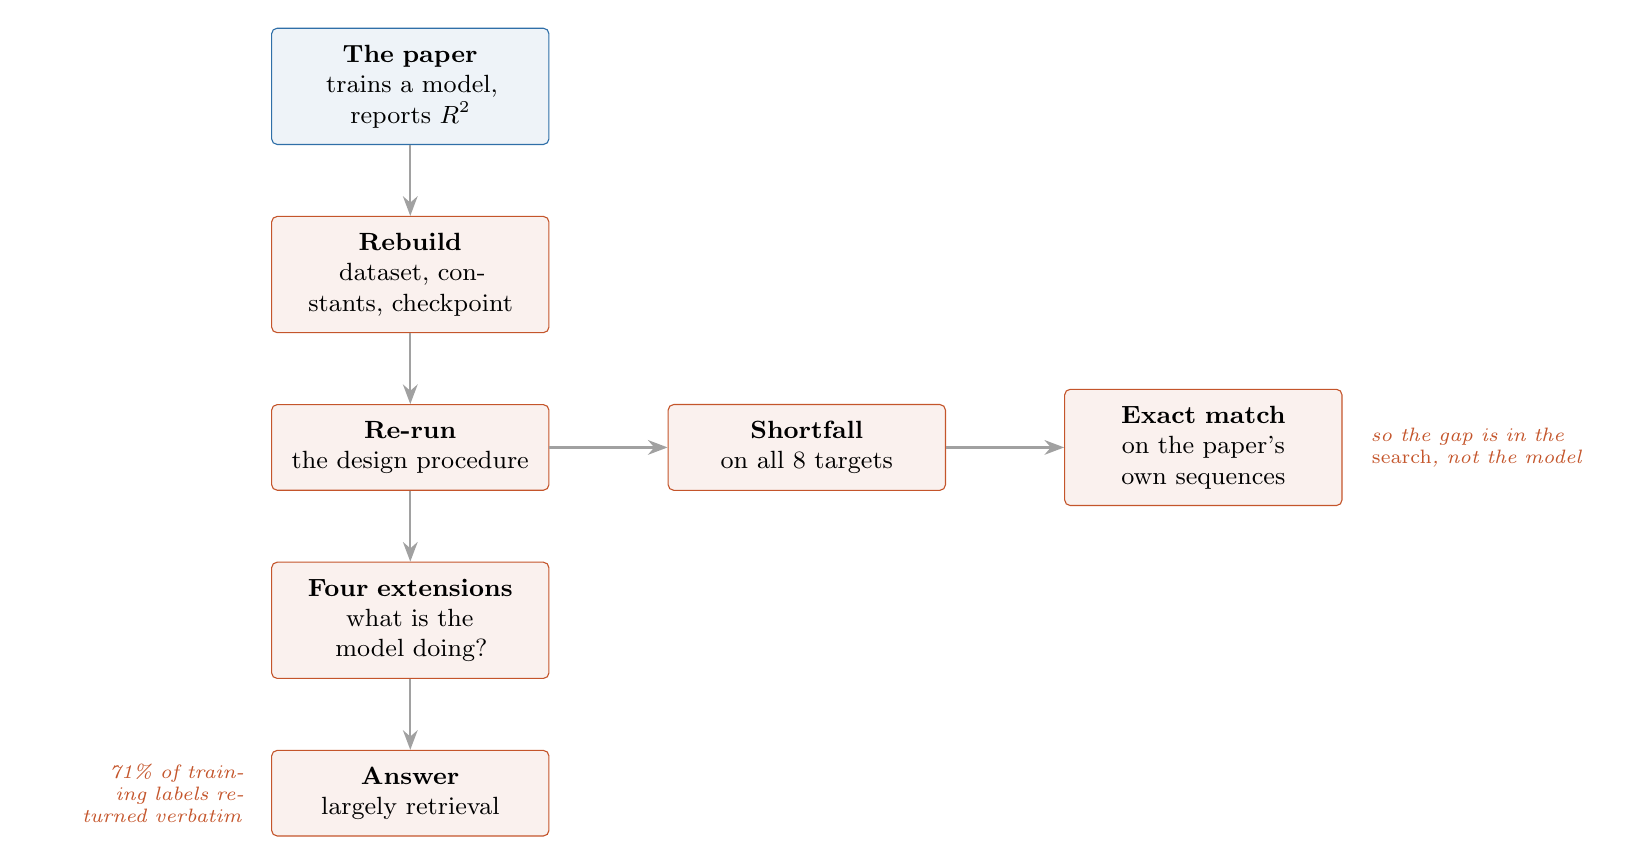
\begin{tikzpicture}[
  font=\small,
  box/.style={draw=greyc!70,fill=boxbg,rounded corners=2pt,inner sep=6pt,
              text width=3.1cm,align=center,minimum height=1.0cm},
  pbox/.style={box,draw=papercol,fill=papercol!8},
  obox/.style={box,draw=ourscol,fill=ourscol!8},
  ar/.style={-{Stealth[length=2.5mm]},thick,greyc!80},
]
\node[pbox] (paper) {\textbf{The paper}\\ trains a model, reports \Rsq};
\node[obox,below=0.9cm of paper] (rebuild) {\textbf{Rebuild}\\ dataset, constants, checkpoint};
\node[obox,below=0.9cm of rebuild] (repro) {\textbf{Re-run}\\ the design procedure};
\node[obox,right=1.5cm of repro] (short) {\textbf{Shortfall}\\ on all 8 targets};
\node[obox,right=1.5cm of short] (exact) {\textbf{Exact match}\\ on the paper's own sequences};
\node[obox,below=0.9cm of repro] (ext) {\textbf{Four extensions}\\ what is the model doing?};
\node[obox,below=0.9cm of ext] (mem) {\textbf{Answer}\\ largely retrieval};

\draw[ar] (paper) -- (rebuild);
\draw[ar] (rebuild) -- (repro);
\draw[ar] (repro) -- (short);
\draw[ar] (short) -- (exact);
\draw[ar] (repro) -- (ext);
\draw[ar] (ext) -- (mem);

\node[right=0.25cm of exact,text width=3.0cm,align=left,font=\scriptsize\itshape,
      text=ourscol]
  {so the gap is in the \emph{search}, not the model};
\node[left=0.25cm of mem,text width=2.6cm,align=right,font=\scriptsize\itshape,
      text=ourscol]
  {71\% of training labels returned verbatim};
\end{tikzpicture}
\caption[Roadmap]{The argument in one figure. Blue is the original paper;
orange is this project. Read it again after Chapter~\ref{ch:paper}.}
\label{fig:roadmap}
\end{figure}

\section{Conventions used throughout}

\begin{itemize}[leftmargin=*,itemsep=2pt]
  \item \paperterm{Blue bold} marks something belonging to the original paper.
  \item \ourterm{Orange bold} marks something this project added or decided.
  \item Amino-acid sequences are set as \aaseq{GAGAGSGAAG}.
  \item Every number I quote as a result was produced by a script in the
        project and is traceable to a file; the mapping is in
        Chapter~\ref{ch:reference}.
\end{itemize}

Three kinds of highlighted box appear:

\begin{keybox}{A concept box looks like this}
Used for definitions and for ideas that need to be held in mind for several
pages.
\end{keybox}

\begin{warnbox}{A caution box looks like this}
Used for traps, for things I got wrong, and for places where a number is easy
to over-read.
\end{warnbox}

\begin{goodbox}{A result box looks like this}
Used for measured outcomes.
\end{goodbox}

\section{A note on the three retractions}

Three times in this project I stated something, and it was wrong, and I had to
withdraw it. They are not hidden in a footnote --- Chapter~\ref{ch:mistakes} is
about them, because they turned out to be the most transferable thing I
learned. Briefly, they were:

\begin{enumerate}[leftmargin=*,itemsep=3pt]
  \item A claim that three of the paper's motif definitions contradicted the
        source they cite. \term{Cause:} I read a two-column PDF table as
        linear text, and the columns interleaved.
  \item A set of \Rsq{} values suggesting the paper's model failed on the
        paper's own sequences. \term{Cause:} my extraction of those sequences
        was silently corrupt, in a way that made every length come out right.
  \item A finding that a composition analysis recovered 12 of 14 published
        residues. \term{Cause:} the selection rule could not fail; random
        noise scored better.
\end{enumerate}

The pattern is the useful part. All three survived internal consistency
checks and all three were caught by comparison against an \emph{external}
published quantity that had played no part in generating the claim.

\chapter{Spider silk, from first principles}
\label{ch:biology}

\section{What a protein is}

A protein is a chain. Each link in the chain is an \term{amino acid}, and there
are twenty different kinds that living things routinely use. Chemistry aside,
the only thing that matters for these notes is this: a protein can be written
down as a string of letters, one letter per link, drawn from a
twenty-letter alphabet.

\begin{center}
\aaseq{M K H T I G I L G G M G P A A T A D M L E K \dots}
\end{center}

The twenty letters, with the names worth knowing for silk:

\begin{center}
\small
\begin{tabular}{llllll}
\toprule
A alanine & C cysteine & D aspartate & E glutamate & F phenylalanine & G glycine \\
H histidine & I isoleucine & K lysine & L leucine & M methionine & N asparagine \\
P proline & Q glutamine & R arginine & S serine & T threonine & V valine \\
W tryptophan & Y tyrosine & & & & \\
\bottomrule
\end{tabular}
\end{center}

A chain of a few hundred of these folds up into a three-dimensional shape, and
the shape plus the chemistry determines what the protein does. For silk, the
relevant consequence is mechanical: how the chains pack together determines how
strong and how stretchy the resulting fibre is.

\begin{keybox}{The central premise of the whole field}
The sequence determines the structure, and the structure determines the
properties. So in principle, if you could learn the map from
\emph{letters} to \emph{mechanical properties}, you could design a fibre by
choosing letters. That map is what the paper tries to learn. Whether it
succeeded, and in what sense, is what this project is about.
\end{keybox}

\section{Why spider silk specifically}

Spider dragline silk --- the stuff a spider hangs from, and the radial spokes
of a web --- has an unusual combination of properties. It is roughly as strong
as steel by weight, far stretchier, and therefore absorbs much more energy
before breaking. That last quantity, energy absorbed per unit volume, is called
\term{toughness}, and it is the property spider silk is famous for.

Four mechanical properties recur throughout this project. They are all read off
a single experiment: take a fibre, pull it until it snaps, and record force
against extension.

\begin{figure}[htbp]
\centering
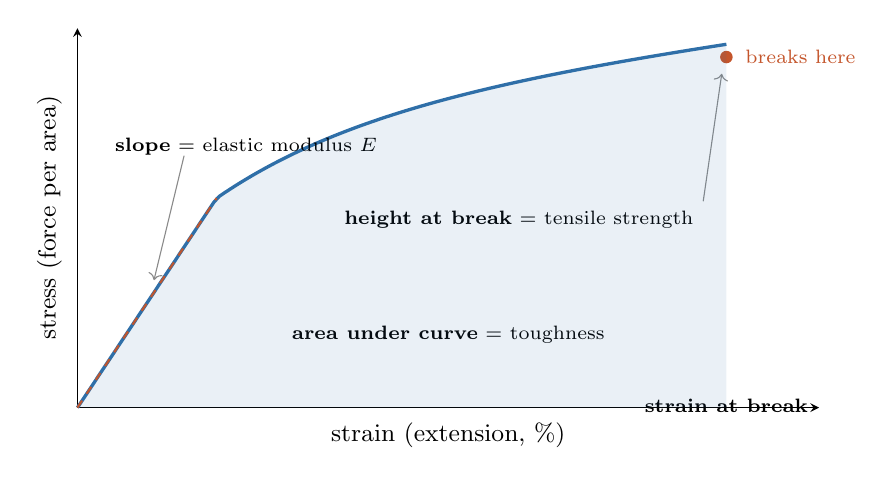
\begin{tikzpicture}[font=\small]
\begin{axis}[
  width=11cm, height=6.4cm,
  xlabel={strain (extension, \%)},
  ylabel={stress (force per area)},
  xmin=0,xmax=32,ymin=0,ymax=1.25,
  axis lines=left, xtick=\empty, ytick=\empty,
  every axis plot/.append style={thick},
  clip=false,
]
\addplot[papercol,line width=1.2pt,domain=0:28,samples=120]
  {x<6 ? 0.115*x : 0.69 + 0.30*(1-exp(-(x-6)/7)) + 0.010*(x-6)};
\addplot[ourscol,dashed,line width=0.8pt] coordinates {(0,0) (6,0.69)};

% breaking point
\node[circle,fill=ourscol,inner sep=1.6pt] at (axis cs:28,1.155) {};
\node[anchor=west,font=\scriptsize,text=ourscol] at (axis cs:28.4,1.155)
  {breaks here};

% annotations
\node[anchor=west,font=\scriptsize] at (axis cs:1.2,0.86)
  {\textbf{slope} $=$ elastic modulus $E$};
\draw[->,greyc,thin] (axis cs:4.6,0.83) -- (axis cs:3.3,0.42);

\node[anchor=east,font=\scriptsize] at (axis cs:27,0.62)
  {\textbf{height at break} $=$ tensile strength};
\draw[->,greyc,thin] (axis cs:27,0.68) -- (axis cs:27.8,1.10);

\node[anchor=north,font=\scriptsize] at (axis cs:16,0.30)
  {\textbf{area under curve} $=$ toughness};

\node[anchor=north,font=\scriptsize] at (axis cs:28,0.06)
  {\textbf{strain at break}};

\addplot[fill=papercol,opacity=0.10,draw=none,domain=0:28,samples=120]
  {x<6 ? 0.115*x : 0.69 + 0.30*(1-exp(-(x-6)/7)) + 0.010*(x-6)} \closedcycle;
\end{axis}
\end{tikzpicture}
\caption[Stress--strain curve]{A stress--strain curve, and where the four
mechanical properties come from. Pull a fibre until it snaps. The initial
\emph{slope} is stiffness (elastic modulus $E$); the \emph{height} at failure
is tensile strength; the \emph{horizontal position} of failure is strain at
break; the \emph{shaded area} is toughness, the energy the fibre absorbed. All
four come from one test, which is why they appear together in the dataset.}
\label{fig:stressstrain}
\end{figure}

\begin{keybox}{The four properties, and why there are eight numbers}
\begin{description}[leftmargin=2.6cm,style=nextline,itemsep=2pt]
  \item[Toughness] Energy absorbed per unit volume before breaking. The area
        under the curve. Units GJ/m$^3$.
  \item[Elastic modulus $E$] Stiffness: how much force to stretch it a little.
        The initial slope. Units GPa.
  \item[Tensile strength] The maximum stress it withstands. Units GPa.
  \item[Strain at break] How far it stretches before failing, as a percentage.
\end{description}
Each is measured several times on fibres from the same spider, so each also has
a \term{standard deviation} --- a measure of how much the repeat measurements
disagreed. Four properties plus four standard deviations makes the
\term{eight-dimensional property vector} that runs through this entire project.
\end{keybox}

The standard deviations are not decoration. A spider's dragline is not made of
one protein but of several, in proportions nobody fully knows, so the same
sequence can be associated with fibres that test differently. Including the
spread is the authors' way of carrying that uncertainty into the model.

\section{Spidroins, and the hierarchy that makes silk work}

The proteins in spider silk are called \term{spidroins}. A spider makes several
families of them from different glands, for different jobs:

\begin{center}
\small
\begin{tabular}{lll}
\toprule
\textbf{Family} & \textbf{Full name} & \textbf{Job} \\
\midrule
\textbf{MaSp} & major ampullate spidroin & dragline; web spokes. \emph{The subject of this paper.} \\
MiSp & minor ampullate spidroin & auxiliary spiral \\
Flag & flagelliform spidroin & the stretchy capture spiral \\
AcSp & aciniform spidroin & prey wrapping, egg-sac lining \\
AgSp & aggregate spidroin & the sticky glue coating \\
PySp & pyriform spidroin & attachment cement \\
CySp & cylindriform (tubuliform) & egg-sac outer wall \\
\bottomrule
\end{tabular}
\end{center}

MaSp is the one that matters here, because dragline silk is what gets
mechanically tested. The paper trains on MaSp only, and one of my extensions
(Section~\ref{sec:nonmasp}) asks what the model does when handed the others.

A spidroin has a characteristic layout, and the layout explains the mechanics.

\begin{figure}[htbp]
\centering
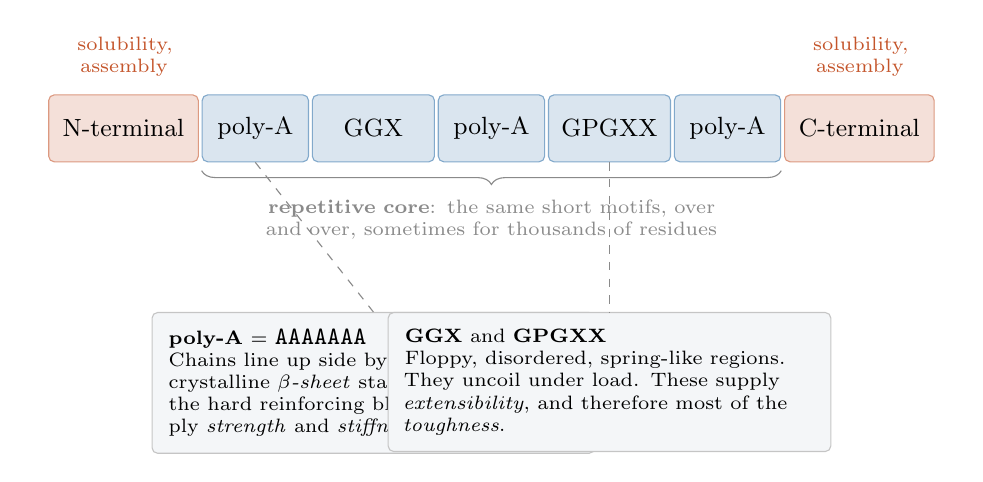
\begin{tikzpicture}[font=\small,
  dom/.style={draw=greyc!70,rounded corners=2pt,minimum height=0.85cm},
  rep/.style={dom,fill=papercol!18,draw=papercol!60},
  nt/.style={dom,fill=ourscol!18,draw=ourscol!60},
]
% the chain
\node[nt,minimum width=1.9cm] (n) at (0,0) {N-terminal};
\node[rep,minimum width=1.35cm,right=1pt of n] (r1) {poly-A};
\node[rep,minimum width=1.55cm,right=1pt of r1] (r2) {GGX};
\node[rep,minimum width=1.35cm,right=1pt of r2] (r3) {poly-A};
\node[rep,minimum width=1.55cm,right=1pt of r3] (r4) {GPGXX};
\node[rep,minimum width=1.35cm,right=1pt of r4] (r5) {poly-A};
\node[nt,minimum width=1.9cm,right=1pt of r5] (c) {C-terminal};

\draw[decorate,decoration={brace,amplitude=5pt,mirror},greyc]
  ($(r1.south west)+(0,-3pt)$) -- ($(r5.south east)+(0,-3pt)$)
  node[midway,below=7pt,font=\scriptsize,text width=6cm,align=center]
  {\textbf{repetitive core}: the same short motifs, over and over, sometimes
   for thousands of residues};

\node[above=3pt of n,font=\scriptsize,text width=2.2cm,align=center,text=ourscol]
  {solubility,\\ assembly};
\node[above=3pt of c,font=\scriptsize,text width=2.2cm,align=center,text=ourscol]
  {solubility,\\ assembly};

% zoom: what polyA and GGX do
\node[draw=greyc!50,fill=boxbg,rounded corners=2pt,inner sep=6pt,
      text width=5.2cm,align=left,font=\scriptsize,below=1.9cm of r2.south]
  (z1) {\textbf{poly-A} $=$ \aaseq{AAAAAAA}\\
        Chains line up side by side into rigid, crystalline
        \emph{$\beta$-sheet} stacks. These are the hard reinforcing
        blocks. They supply \emph{strength} and \emph{stiffness}.};
\node[draw=greyc!50,fill=boxbg,rounded corners=2pt,inner sep=6pt,
      text width=5.2cm,align=left,font=\scriptsize,below=1.9cm of r4.south]
  (z2) {\textbf{GGX} and \textbf{GPGXX}\\
        Floppy, disordered, spring-like regions. They uncoil under load.
        These supply \emph{extensibility}, and therefore most of the
        \emph{toughness}.};
\draw[greyc,thin,dashed] (r1.south) -- (z1.north);
\draw[greyc,thin,dashed] (r4.south) -- (z2.north);
\end{tikzpicture}
\caption[Spidroin layout]{The layout of a spidroin. Two non-repetitive terminal
domains bracket a long repetitive core. The core alternates hard crystalline
blocks with soft extensible ones. ``X'' stands for a position that varies.}
\label{fig:spidroin}
\end{figure}

\begin{keybox}{The analogy that makes silk make sense}
Think of a rope made of rubber bands with steel beads threaded on at intervals.
The steel beads (poly-alanine $\beta$-sheets) stop it from pulling apart --- they
give strength. The rubber (GGX, GPGXX) lets it stretch a long way before
anything breaks --- it gives extensibility. Toughness, the energy absorbed, is
strength \emph{times} extensibility, roughly, which is why you need both, and
why silk beats materials that have only one.
\end{keybox}

This is why the ablation experiment in Section~\ref{sec:ablations} deletes
poly-A tracts specifically. If the model has learned anything mechanically
meaningful, removing the hard blocks should change its predictions about
strength and stiffness. Whether it does is one of the project's main findings.

\section{The Silkome dataset}
\label{sec:silkome}

Everything downstream depends on one dataset, so it is worth being precise
about what is in it.

\begin{keybox}{Silkome}
Arakawa \emph{et al.}, ``1000 spider silkomes: linking sequences to silk
physical properties'', \emph{Science Advances} \textbf{8}, eabo6043 (2022).

Two files matter:
\begin{itemize}[leftmargin=*,itemsep=2pt]
  \item \code{spider-silkome-database.v1.prot.fasta} --- 11{,}155 spidroin
        sequence records across many species.
  \item \code{mechanical\_properties.csv} --- 446 rows, one per individual
        spider whose dragline was pulled apart in a testing machine.
\end{itemize}
\end{keybox}

Two features of this dataset caused me real work later.

\paragraph{The sequences are terminal-domain records, not whole proteins.}
Each FASTA record is labelled \code{NTD} or \code{CTD}, meaning it is anchored
on the N- or C-terminal domain and runs some distance into the repetitive core.
A full spidroin can be several thousand residues; these records are typically
a few hundred. So when the paper says it trains on ``sequences'', it means
these fragments.

\paragraph{Properties belong to spiders, sequences belong to genes.}
A single spider yields many sequence records --- MaSp1, MaSp2, MiSp, Flag and so
on, each NTD and CTD --- but only \emph{one} set of mechanical measurements,
taken on its dragline. So the join between the two files is one-to-many, and
the key is the individual spider. Getting this wrong is what made my first
attempt at rebuilding the dataset return zero rows
(Section~\ref{sec:dataset}).

\begin{warnbox}{A consequence worth carrying forward}
Because the mechanical test is done on \emph{dragline}, and dragline is made of
\emph{MaSp}, a Flag sequence in this dataset is paired with the mechanical
properties of the same spider's dragline --- not of its flagelliform silk. The
paper is explicit about assuming ``MaSp governs the mechanics'', and restricting
to MaSp follows from that. It also means the out-of-distribution experiment in
Section~\ref{sec:nonmasp} has to be phrased carefully: no analysis of this
dataset could tell you whether a model predicts flagelliform properties,
because the dataset does not contain them.
\end{warnbox}

\chapter{Language models, from first principles}
\label{ch:transformers}

This chapter builds up exactly enough machinery to understand what SilkomeGPT
is. If you already know what a decoder-only transformer is, skip to
Section~\ref{sec:decoding}, which covers the decoding settings --- those turn
out to matter more for this project than the architecture does.

\section{The one thing a language model does}

A language model does one thing: given a piece of text, it assigns a
probability to every possible next chunk of text.

That is genuinely all. Everything else --- chat, translation, protein design ---
is built by choosing what to put in and how to read what comes out.

Write the input as a sequence of tokens $t_1, t_2, \dots, t_n$. The model
computes
\[
  P(t_{n+1} \mid t_1, \dots, t_n)
\]
a probability for each of the $\approx$50{,}000 possible next tokens. To
generate text you sample one from that distribution, append it, and repeat.
This is called \term{autoregressive} generation: each new token is conditioned
on everything already written, including what the model itself just wrote.

\begin{keybox}{Why this is enough to design proteins}
If you train the model on text of the form
\begin{center}
\code{[a description of what I want][the protein that satisfies it]}
\end{center}
then at generation time you write the description, and the machinery that
predicts ``the most likely continuation'' has no choice but to produce a
protein that fits it. Design becomes autocomplete. The trick is entirely in the
format of the training text.
\end{keybox}

\section{Tokens: how text becomes numbers}

Neural networks consume numbers, not letters. A \term{tokenizer} chops text
into pieces and assigns each piece an integer ID. The \term{vocabulary} is the
set of pieces it knows.

The naive choice for proteins is one token per amino acid, giving a vocabulary
of twenty. SilkomeGPT does something more efficient, called \term{byte-pair
encoding} (BPE), and the reason matters for silk in particular.

\begin{keybox}{Byte-pair encoding, by example}
BPE learns its vocabulary from data by repeatedly merging the most frequent
adjacent pair. Suppose the training data is full of the fragment
\aaseq{GAGAGA}. Then:

\begin{enumerate}[leftmargin=*,itemsep=1pt]
  \item Start with single letters: \aaseq{G}, \aaseq{A}.
  \item \aaseq{G}+\aaseq{A} is the most frequent adjacent pair $\rightarrow$
        merge into a new token \aaseq{GA}.
  \item Now \aaseq{GA}+\aaseq{GA} is frequent $\rightarrow$ merge into
        \aaseq{GAGA}.
  \item Continue until the vocabulary reaches the target size.
\end{enumerate}

The result: common motifs become \emph{single tokens}. A poly-alanine run
\aaseq{AAAAAAAA} might be one token rather than eight.
\end{keybox}

This is why the numbers in this project look odd at first glance. The paper's
worked-example sequence is 635 amino acids long but only 198 tokens. That is
about 3.2 residues per token, and it happens because spidroins are extremely
repetitive --- exactly the situation BPE compresses well. SilkomeGPT's tokenizer
was trained on $\approx$800{,}000 protein sequences with a vocabulary of up to
50{,}000.

\begin{warnbox}{A trap this creates}
Because compression depends on how repetitive a sequence is, token count is not
proportional to residue count. A highly repetitive 2000-residue spidroin may
tokenise to fewer tokens than a non-repetitive 800-residue one. Any reasoning
about ``context limits'' has to be done in tokens, not residues.
\end{warnbox}

\section{Attention, and what makes a transformer}

The architecture underneath is a \term{transformer}. Its central mechanism is
\term{self-attention}, and the idea is simpler than its reputation.

When the model processes a token, it needs context from other tokens. Attention
lets every position look at every other position and decide how much each one
matters, for this particular purpose, right now.

\begin{figure}[htbp]
\centering
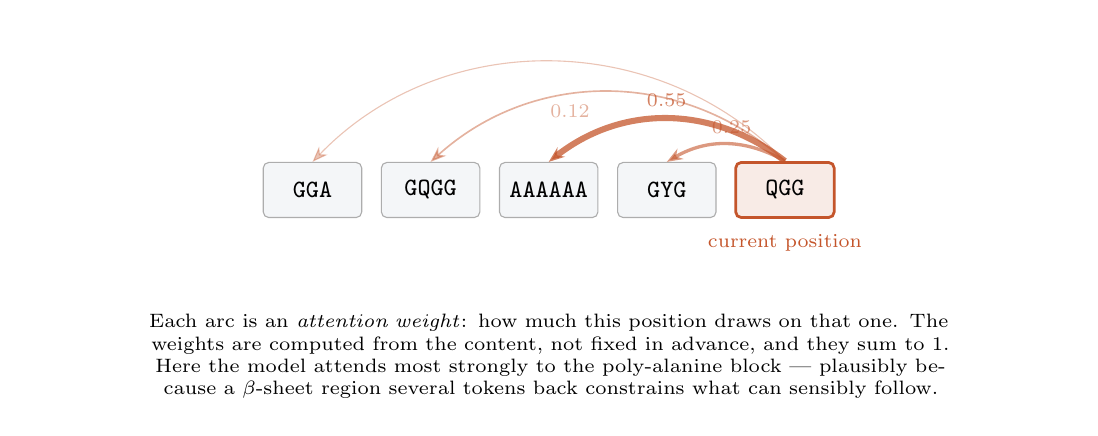
\begin{tikzpicture}[font=\small,
  tok/.style={draw=greyc!70,fill=boxbg,rounded corners=2pt,
              minimum width=1.25cm,minimum height=0.7cm},
  cur/.style={tok,draw=ourscol,fill=ourscol!12,line width=1pt},
]
\node[tok] (t1) at (0,0)   {\aaseq{GGA}};
\node[tok] (t2) at (1.5,0) {\aaseq{GQGG}};
\node[tok] (t3) at (3.0,0) {\aaseq{AAAAAA}};
\node[tok] (t4) at (4.5,0) {\aaseq{GYG}};
\node[cur] (t5) at (6.0,0) {\aaseq{QGG}};

\node[font=\scriptsize,below=2pt of t5,text=ourscol]
  {current position};

% attention arcs, thickness = weight
\draw[-{Stealth[length=2mm]},ourscol,line width=2.2pt,opacity=0.75]
  (t5.north) to[bend right=38] node[above,font=\scriptsize,pos=0.5]{0.55} (t3.north);
\draw[-{Stealth[length=2mm]},ourscol,line width=1.2pt,opacity=0.6]
  (t5.north) to[bend right=30] node[above,font=\scriptsize,pos=0.45]{0.25} (t4.north);
\draw[-{Stealth[length=2mm]},ourscol,line width=0.6pt,opacity=0.45]
  (t5.north) to[bend right=42] node[below,font=\scriptsize,pos=0.6]{0.12} (t2.north);
\draw[-{Stealth[length=2mm]},ourscol,line width=0.4pt,opacity=0.35]
  (t5.north) to[bend right=46] (t1.north);

\node[text width=13cm,align=center,font=\scriptsize,below=1.1cm of t3]
  {Each arc is an \emph{attention weight}: how much this position draws on that
   one. The weights are computed from the content, not fixed in advance, and
   they sum to 1. Here the model attends most strongly to the poly-alanine
   block --- plausibly because a $\beta$-sheet region several tokens back
   constrains what can sensibly follow.};
\end{tikzpicture}
\caption[Attention]{Self-attention at one position. Thickness indicates weight.
Because weights are recomputed from content at every position, the model can
route information over arbitrary distances --- which is what lets it connect a
crystalline block to a distant terminal domain.}
\label{fig:attention}
\end{figure}

Three further pieces complete the picture:

\begin{description}[leftmargin=0cm,style=nextline,itemsep=4pt]
\item[Multi-head attention.] The above is done several times in parallel with
  different learned projections --- SilkomeGPT uses \paperterm{8 heads}. One head
  might track repeat periodicity, another composition, another distance to the
  terminal domain. They are concatenated.

\item[Layers.] The whole operation (attention, then a small feed-forward
  network) is stacked. SilkomeGPT has \paperterm{12 layers}. Early layers
  handle local patterns; later layers combine them into longer-range structure.

\item[Positional information.] Attention alone is order-blind --- it sees a bag
  of tokens. Position must be injected. SilkomeGPT uses \term{rotary positional
  embeddings} (RoPE), which encode position by rotating each token's vector by
  an angle proportional to its index. The useful property is that the
  \emph{relative} offset between two positions is what survives into the
  attention computation, so patterns learned at one place transfer to another
  --- well suited to a protein made of the same motif repeated at many offsets.
\end{description}

\begin{figure}[htbp]
\centering
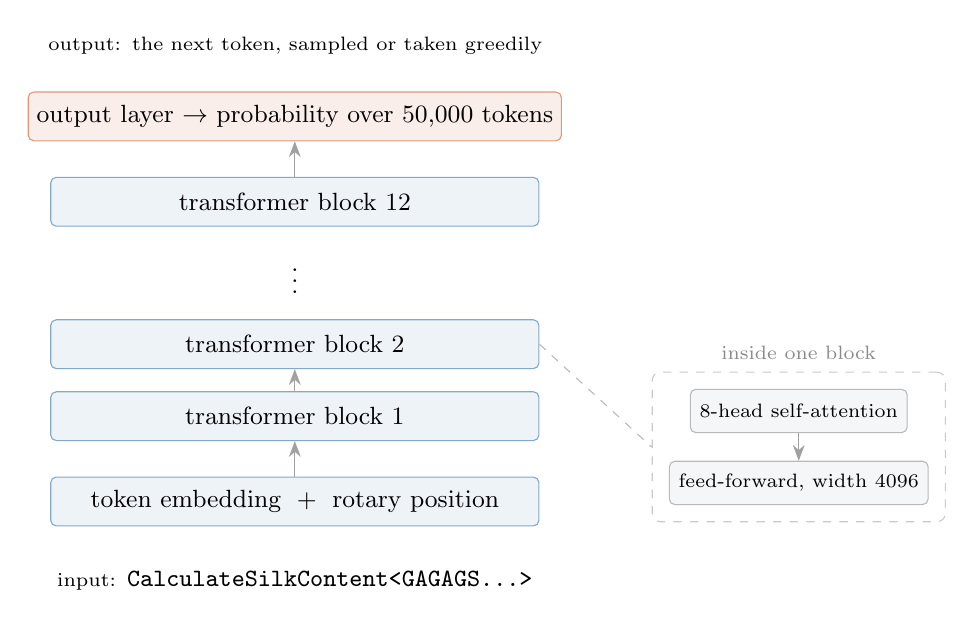
\begin{tikzpicture}[font=\small,
  lay/.style={draw=papercol!60,fill=papercol!8,rounded corners=2pt,
              minimum width=6.2cm,minimum height=0.62cm,inner sep=3pt},
  sub/.style={draw=greyc!60,fill=boxbg,rounded corners=2pt,
              minimum width=2.7cm,minimum height=0.55cm,font=\scriptsize},
  ar/.style={-{Stealth[length=2mm]},greyc!80},
]
\node[lay] (emb) at (0,0) {token embedding \;+\; rotary position};
\node[lay,above=0.45cm of emb] (l1) {transformer block 1};
\node[lay,above=0.28cm of l1] (l2) {transformer block 2};
\node[above=0.20cm of l2,font=\small] (dots) {$\vdots$};
\node[lay,above=0.20cm of dots] (l12) {transformer block 12};
\node[lay,above=0.45cm of l12,fill=ourscol!10,draw=ourscol!60] (head)
  {output layer $\rightarrow$ probability over 50{,}000 tokens};

\draw[ar] (emb) -- (l1);
\draw[ar] (l1) -- (l2);
\draw[ar] (l12) -- (head);

% expansion of one block
\node[sub] (att) at (6.4,1.15) {8-head self-attention};
\node[sub,below=0.35cm of att] (ff) {feed-forward, width 4096};
\draw[ar] (att) -- (ff);
\node[draw=greyc!45,dashed,rounded corners=3pt,
      fit=(att)(ff),inner sep=6pt] (blk) {};
\node[above=1pt of blk,font=\scriptsize,text=greyc] {inside one block};
\draw[greyc!60,dashed] (l2.east) -- (blk.west);

\node[below=0.45cm of emb,font=\scriptsize,text width=6.4cm,align=center]
  {input: \code{CalculateSilkContent<GAGAGS\dots>}};
\node[above=0.35cm of head,font=\scriptsize,text width=6.4cm,align=center]
  {output: the next token, sampled or taken greedily};
\end{tikzpicture}
\caption[Architecture]{SilkomeGPT's architecture. Hidden width 1024,
feed-forward width 4096, 12 blocks, 8 heads --- 253{,}556{,}736 parameters in
total. ``Decoder-only'' means there is just this one stack: no separate encoder,
and each position may attend only to positions before it.}
\label{fig:arch}
\end{figure}

\begin{keybox}{Parameters}
A \term{parameter} is one learned number. SilkomeGPT has 253.6 million of them.
Training means adjusting all of them so that the model's predicted
next-token probabilities match what actually came next in the training data.
Verifying that the released model really has this many, and in this
arrangement, was the first check I ran (Section~\ref{sec:checkpoint}).
\end{keybox}

\section{Pretraining and fine-tuning}

Training happened in two stages, and the distinction matters for interpreting
the results.

\begin{description}[leftmargin=0cm,style=nextline,itemsep=5pt]
\item[Pretraining.] The model saw $\approx$600{,}000 protein sequences from
  across biology and learned to predict the next token. No properties involved.
  The point is to absorb the general statistics of proteins --- which residues
  follow which, what real sequences look like.

\item[Fine-tuning.] The model was then trained further on the 1{,}033 silk
  sequences \emph{paired with their measured properties}, in a specific text
  format. This is where the property knowledge enters.
\end{description}

\begin{warnbox}{The fact that shapes every later interpretation}
The paper states that fine-tuning used ``all known pairs of sequence and
properties''. There is no \term{held-out set} --- no sequences kept aside to
test on. Every one of the 1{,}033 pairs was seen during training.

This is not a mistake; with 1{,}033 examples you want to use all of them, and
the paper reports self-consistency rather than predictive accuracy. But it means
no number measured on those 1{,}033 pairs can distinguish \emph{learning} from
\emph{memorising}. Chapter~\ref{ch:extensions} shows that the distinction is
not academic here.
\end{warnbox}

\section{Decoding: turning probabilities into text}
\label{sec:decoding}

The model outputs a probability for each possible next token. Turning that into
an actual choice is called \term{decoding}, and the settings involved caused
more subtlety in this project than anything in the architecture.

\begin{description}[leftmargin=0cm,style=nextline,itemsep=5pt]
\item[Greedy decoding.] Always take the highest-probability token.
  Deterministic: the same input always gives the same output.

\item[Sampling.] Draw randomly according to the probabilities. Different every
  time. Necessary for generating variety.

\item[Temperature $T$.] Rescales the distribution before sampling.
  $T \to 0$ approaches greedy; $T = 1$ samples from the raw distribution;
  $T > 1$ flattens it, making unlikely tokens more likely. The paper's inverse
  task uses $T = 1.25$ --- deliberately adventurous, because it wants novel
  designs.

\item[top-$k$ and top-$p$.] Truncation rules. top-$k$ keeps only the $k$ most
  likely tokens; top-$p$ (nucleus sampling) keeps the smallest set whose
  probabilities sum to $p$. Both stop the model from occasionally emitting
  something absurd.
\end{description}

\begin{figure}[htbp]
\centering
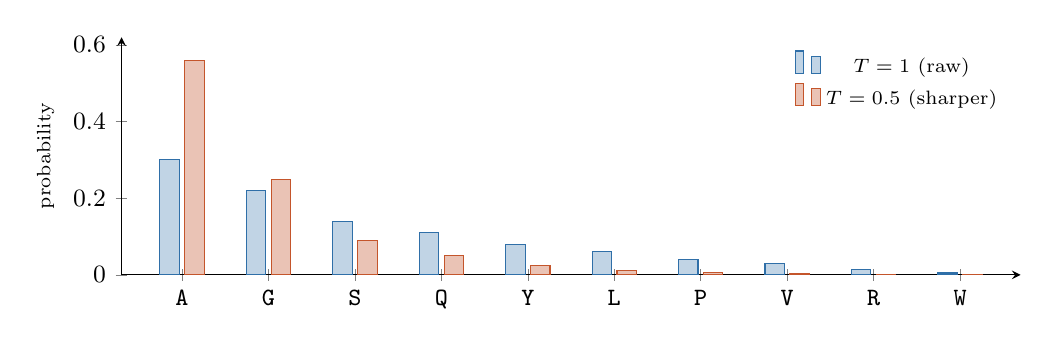
\begin{tikzpicture}[font=\small]
\begin{axis}[
  width=13cm,height=4.6cm,
  ybar, bar width=7pt,
  ymin=0,ymax=0.62, xmin=0.3, xmax=10.7,
  xtick={1,...,10},
  xticklabels={\aaseq{A},\aaseq{G},\aaseq{S},\aaseq{Q},\aaseq{Y},\aaseq{L},\aaseq{P},\aaseq{V},\aaseq{R},\aaseq{W}},
  ylabel={probability},
  axis lines=left, ylabel style={font=\scriptsize},
  legend style={font=\scriptsize,draw=none,at={(0.99,0.97)},anchor=north east},
]
\addplot[fill=papercol!30,draw=papercol] coordinates
  {(1,0.30)(2,0.22)(3,0.14)(4,0.11)(5,0.08)(6,0.06)(7,0.04)(8,0.03)(9,0.015)(10,0.005)};
\addlegendentry{$T=1$ (raw)}
\addplot[fill=ourscol!35,draw=ourscol] coordinates
  {(1,0.56)(2,0.25)(3,0.09)(4,0.05)(5,0.025)(6,0.012)(7,0.007)(8,0.004)(9,0.001)(10,0.0003)};
\addlegendentry{$T=0.5$ (sharper)}
\end{axis}
\end{tikzpicture}
\caption[Temperature]{Temperature reshapes the next-token distribution.
Lowering $T$ concentrates mass on the leader, making output more predictable
and less varied; raising it does the opposite. At $T \to 0$ sampling becomes
greedy decoding.}
\label{fig:temperature}
\end{figure}

\begin{keybox}{The settings used in this project}
\begin{center}
\small
\begin{tabular}{lcccc}
\toprule
& temperature & top-$k$ & top-$p$ & max new tokens \\
\midrule
inverse task (design) & 1.25 & 500 & 0.8 & 512 \\
forward task (predict), \paperterm{paper} & 0.01 & 500 & 0.9 & 64 \\
forward task (predict), \ourterm{ours} & \multicolumn{3}{c}{greedy} & 64 \\
\bottomrule
\end{tabular}
\end{center}
None of these appear in the paper; all were read out of the authors' released
notebook. Why I departed from the paper on the forward task, and the
measurements that justified it, is Section~\ref{sec:decodingchoice}.
\end{keybox}

\chapter{\texorpdfstring{$R^2$}{R-squared}, and the trap inside it}
\label{ch:metrics}

Every headline number in the paper is an \Rsq{} value. Almost every subtlety in
this project comes from what those values are computed \emph{over}. This
chapter is therefore not optional background --- it is the key to the whole
thing.

\section{What \texorpdfstring{$R^2$}{R-squared} means}

\Rsq{} answers one question: \emph{how much better are these predictions than
just guessing the average?}

Given true values $y_1,\dots,y_n$ and predictions $\hat{y}_1,\dots,\hat{y}_n$,
let $\bar{y}$ be the mean of the true values. Define

\[
  \mathrm{SS}_{\text{res}} = \sum_{i=1}^{n} (y_i - \hat{y}_i)^2,
  \qquad
  \mathrm{SS}_{\text{tot}} = \sum_{i=1}^{n} (y_i - \bar{y})^2,
\]

\[
  \boxed{\;R^2 = 1 - \frac{\mathrm{SS}_{\text{res}}}{\mathrm{SS}_{\text{tot}}}\;}
\]

$\mathrm{SS}_{\text{res}}$ is how wrong the predictions are.
$\mathrm{SS}_{\text{tot}}$ is how wrong you would be if you always guessed the
mean. The ratio compares the two.

\begin{keybox}{Reading the scale}
\begin{description}[leftmargin=1.6cm,style=nextline,itemsep=1pt]
\item[$R^2 = 1$] Perfect. Every prediction exactly right.
\item[$R^2 = 0$] Exactly as good as always guessing the mean.
\item[$R^2 < 0$] \emph{Worse} than guessing the mean. Entirely possible, and it
  happens frequently in this project.
\end{description}
The negative range surprises people who have only seen \Rsq{} as ``the fraction
of variance explained''. That interpretation holds only for a fitted linear
regression on its own training data. For predictions from anywhere else --- a
neural network, another dataset, a wish list --- there is no lower bound.
\end{keybox}

\section{The trap: \texorpdfstring{$R^2$}{R-squared} over \emph{what}?}
\label{sec:r2trap}

The formula needs a set of pairs. Nothing says what the set is. The paper and
a casual reader can easily mean different things, and here they do.

\begin{figure}[htbp]
\centering
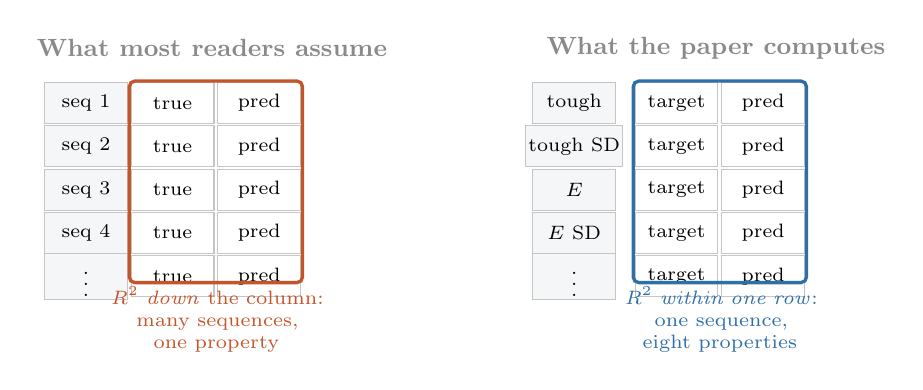
\begin{tikzpicture}[font=\small,
  hdr/.style={font=\small\bfseries},
  cell/.style={draw=greyc!50,minimum width=1.05cm,minimum height=0.52cm,
               font=\scriptsize,inner sep=1pt},
]
% ---------- LEFT: across-dataset ----------
\node[hdr,text=greyc] at (0,3.3) {What most readers assume};
\foreach \i/\lab in {0/seq 1,1/seq 2,2/seq 3,3/seq 4,4/$\vdots$} {
  \node[cell,fill=boxbg] at (-1.6, 2.6-0.55*\i) {\lab};
  \node[cell] at (-0.5, 2.6-0.55*\i) {true};
  \node[cell] at (0.6, 2.6-0.55*\i) {pred};
}
\draw[ourscol,line width=1.2pt,rounded corners=2pt]
  (-1.05,2.88) rectangle (1.15,0.32);
\node[font=\scriptsize,text=ourscol,align=center,text width=3.2cm]
  at (0.05,-0.15)
  {$R^2$ \emph{down} the column:\\ many sequences, one property};

% ---------- RIGHT: within-vector ----------
\node[hdr,text=greyc] at (6.4,3.3) {What the paper computes};
\foreach \i/\lab in {0/tough,1/tough SD,2/$E$,3/$E$ SD,4/$\vdots$} {
  \node[cell,fill=boxbg] at (4.6, 2.6-0.55*\i) {\lab};
  \node[cell] at (5.9, 2.6-0.55*\i) {target};
  \node[cell] at (7.0, 2.6-0.55*\i) {pred};
}
\draw[papercol,line width=1.2pt,rounded corners=2pt]
  (5.35,2.88) rectangle (7.55,0.32);
\node[font=\scriptsize,text=papercol,align=center,text width=3.6cm]
  at (6.45,-0.15)
  {$R^2$ \emph{within one row}:\\ one sequence, eight properties};
\end{tikzpicture}
\caption[Two meanings of R-squared]{The same formula, two completely different
quantities. Left: the standard regression sense --- how well does the model
predict toughness across many sequences? Right: what the paper actually
computes --- for one designed sequence, do its eight predicted property values
match the eight that were requested?}
\label{fig:r2two}
\end{figure}

\subsection{The paper's definition, precisely}

The released notebook makes it unambiguous. Inside the design loop:

\begin{lstlisting}[style=py]
r2 = r2_score(req, prop)   # req: the 8 requested values
                           # prop: the 8 predicted values
\end{lstlisting}

Both arguments have length 8. So $n = 8$, and the eight ``observations'' are the
eight \emph{properties} of a single sequence.

\begin{keybox}{What the paper's \Rsq{} actually measures}
It is a \term{self-consistency} check on a round trip:

\begin{center}
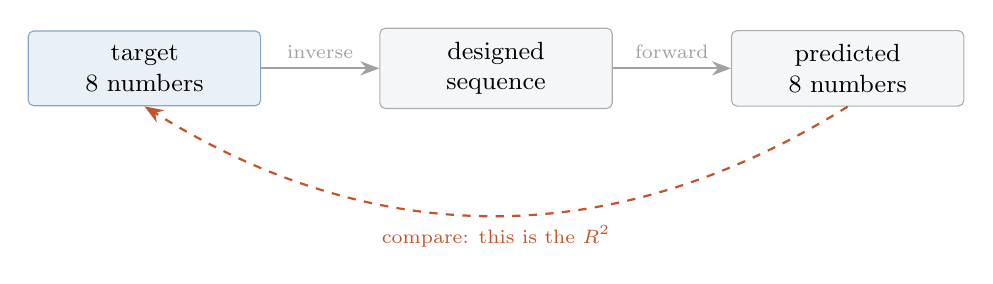
\begin{tikzpicture}[font=\small,
  n/.style={draw=greyc!70,fill=boxbg,rounded corners=2pt,inner sep=5pt,
            text width=2.6cm,align=center,minimum height=0.95cm},
  ar/.style={-{Stealth[length=2.4mm]},thick,greyc!80},
]
\node[n,fill=papercol!10,draw=papercol!60] (t) {target\\ 8 numbers};
\node[n,right=1.5cm of t] (s) {designed\\ sequence};
\node[n,right=1.5cm of s] (p) {predicted\\ 8 numbers};
\draw[ar] (t) -- node[above,font=\scriptsize]{inverse} (s);
\draw[ar] (s) -- node[above,font=\scriptsize]{forward} (p);
\draw[ar,ourscol,dashed] (p.south) to[bend left=32]
  node[below,font=\scriptsize,text=ourscol]{compare: this is the $R^2$} (t.south);
\end{tikzpicture}
\end{center}

It asks: when the model designs a sequence for a target, and is then asked what
that sequence's properties are, does it agree with itself? That is a
meaningful thing to measure, and the paper describes it as such. It is
\emph{not} a measure of whether the sequence really has those properties, and
it is not a measure of generalisation to unseen sequences.
\end{keybox}

\subsection{Two consequences that bite}

\paragraph{The denominator is tiny, and varies between targets.}
$\mathrm{SS}_{\text{tot}}$ is the spread of the \emph{eight target values}. If a
target is $[0.25, 0.252, 0.20, 0.151, 0.31, 0.203, 0.293, 0.265]$ --- all
clustered around $0.25$ --- then the denominator is small, and a modest absolute
error produces a dramatic \Rsq{}. Two targets with the same absolute accuracy
can score very differently purely because one is more spread out. I report this
spread alongside every within-vector \Rsq{} in the project, under the name
\code{target\_spread}.

\paragraph{Half the entries are standard deviations.}
Four of the eight numbers are property values; four are measurement standard
deviations. The SDs vary less across the dataset, so they are easier to predict.
A model that nails the four SDs and misses the four properties still scores
respectably. Throughout the project I therefore report the four mechanical
slots separately, via an index list \code{MECHANICAL\_IDX = [0, 2, 4, 6]}.

\begin{warnbox}{Argument order is not symmetric}
$R^2(a, b) \neq R^2(b, a)$, because the denominator uses the variance of the
\emph{first} argument only. The released notebook uses \code{r2\_score(req,
prop)} --- target first --- in the loop that produces the published numbers, and
\code{r2\_score(c\_res, c\_GT)} --- predictions first --- in a separate helper
that does not appear to feed any published figure. I mention it only because
somebody reusing that helper would be computing a different quantity. This
project always uses (target, prediction), and has a test asserting the two
differ so the convention cannot drift.
\end{warnbox}

\section{Best-of-\texorpdfstring{$N$}{N}: why a maximum is not a measurement}
\label{sec:bestofn-concept}

This is the single most important statistical idea in the project.

Suppose a procedure produces candidates with some spread of quality. Generate
$N$ of them and keep the best. The expected quality of what you keep
\emph{increases with $N$}, without anything about the procedure improving.

\begin{figure}[htbp]
\centering
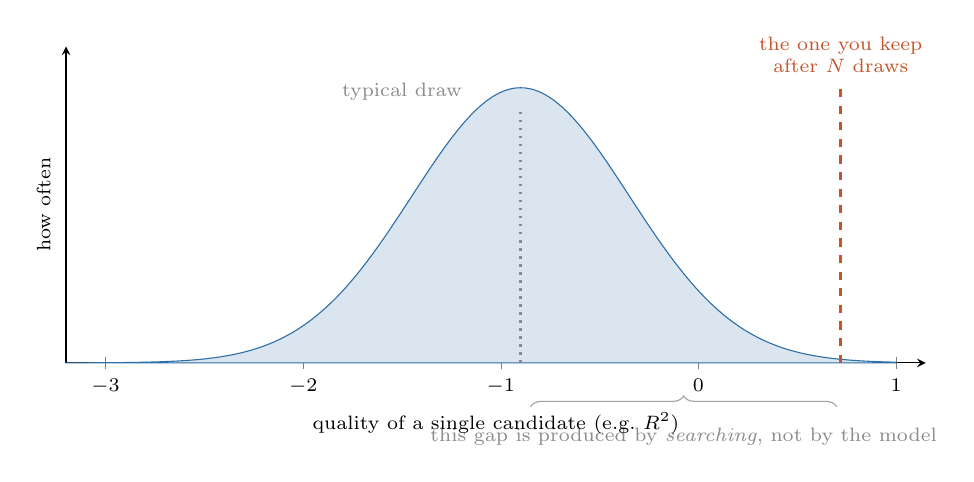
\begin{tikzpicture}[font=\small]
\begin{axis}[
  width=12.5cm,height=5.6cm,
  xlabel={quality of a single candidate (e.g.\ $R^2$)},
  ylabel={how often},
  axis lines=left, ytick=\empty,
  xmin=-3.2,xmax=1.15, ymin=0, ymax=1.15,
  xlabel style={font=\scriptsize}, ylabel style={font=\scriptsize},
  xtick={-3,-2,-1,0,1}, xticklabel style={font=\scriptsize},
  clip=false,
]
\addplot[draw=papercol,fill=papercol!18,domain=-3.2:1.0,samples=200]
  {exp(-((x+0.9)^2)/(2*0.55^2))} \closedcycle;

\draw[ourscol,line width=1.1pt,dashed] (axis cs:0.72,0) -- (axis cs:0.72,1.02);
\node[anchor=south,font=\scriptsize,text=ourscol,align=center]
  at (axis cs:0.72,1.02) {the one you keep\\ after $N$ draws};

\draw[greyc,line width=0.9pt,dotted] (axis cs:-0.9,0) -- (axis cs:-0.9,0.92);
\node[anchor=south,font=\scriptsize,text=greyc] at (axis cs:-1.5,0.92)
  {typical draw};

\draw[decorate,decoration={brace,amplitude=4pt},greyc!80]
  (axis cs:-0.85,-0.16) -- (axis cs:0.70,-0.16)
  node[midway,below=4pt,font=\scriptsize,text=greyc]
  {this gap is produced by \emph{searching}, not by the model};
\end{axis}
\end{tikzpicture}
\caption[Best-of-N]{The best-of-$N$ effect. The shaded curve is the quality of
a single candidate --- mostly poor. Draw many and keep the maximum, and you land
far out in the right tail. Report only the maximum, without $N$, and a reader
cannot tell how much of the number came from the model and how much from the
search.}
\label{fig:bestofn-concept}
\end{figure}

\begin{keybox}{The order statistic}
If a single candidate's quality has cumulative distribution $F$, then the
maximum of $N$ independent draws has distribution
\[
  P(\max \le x) = F(x)^N ,
\]
which pushes steadily rightward as $N$ grows. The expected maximum increases
without bound in $N$ (until it saturates at the distribution's upper limit).
This is a fact about sampling, not about the sampler's competence.
\end{keybox}

\begin{warnbox}{Why this matters here}
The paper reports its \Rsq{} values as ``the results with the highest \Rsq{}
values are selected from a set of sampling attempts''. The size of that set
appears nowhere in the paper. The released notebook shows it: 32 samples per
step $\times$ 64 repeats $=$ up to \textbf{2{,}048 candidates}, then
\code{np.argmax}.

There is nothing wrong with the procedure. If generation is cheap and screening
is cheaper, generating thousands of candidates and keeping the best is exactly
what a practitioner should do. The issue is purely one of reporting: without
$N$, the number cannot be compared against another method's single-shot result,
and a reader cannot estimate the compute needed to reach it.

Quantifying this became Extension~1 (Section~\ref{sec:bestofn}).
\end{warnbox}

\section{In-sample versus held-out, and why it matters here}

A last piece of vocabulary, needed for Chapter~\ref{ch:extensions}.

\begin{description}[leftmargin=0cm,style=nextline,itemsep=4pt]
\item[In-sample.] Performance measured on the data the model was trained on. It
  is an upper bound. A model that simply memorised a lookup table scores
  perfectly in-sample and has learned nothing.

\item[Held-out (out-of-sample).] Performance on data withheld from training.
  This is what tells you whether anything general was learned.
\end{description}

Since SilkomeGPT was fine-tuned on all 1{,}033 pairs, every property-prediction
number measurable on those pairs --- the paper's and mine --- is in-sample. This
does not contradict anything the paper claims, because it does not claim
held-out accuracy. But it means the two possibilities, \emph{learning} and
\emph{memorising}, cannot be told apart from the published figures alone.
Distinguishing them is Extension~4 (Section~\ref{sec:memorisation}), and the
answer is not the comfortable one.

\chapter{What the paper did}
\label{ch:paper}

Everything in this chapter belongs to Lu, Kaplan \& Buehler. My own work starts
in Chapter~\ref{ch:reproduction}.

\section{The three tasks}

Fine-tuning taught the model three text formats. The formats \emph{are} the
interface --- there is no other API.

\begin{figure}[htbp]
\centering
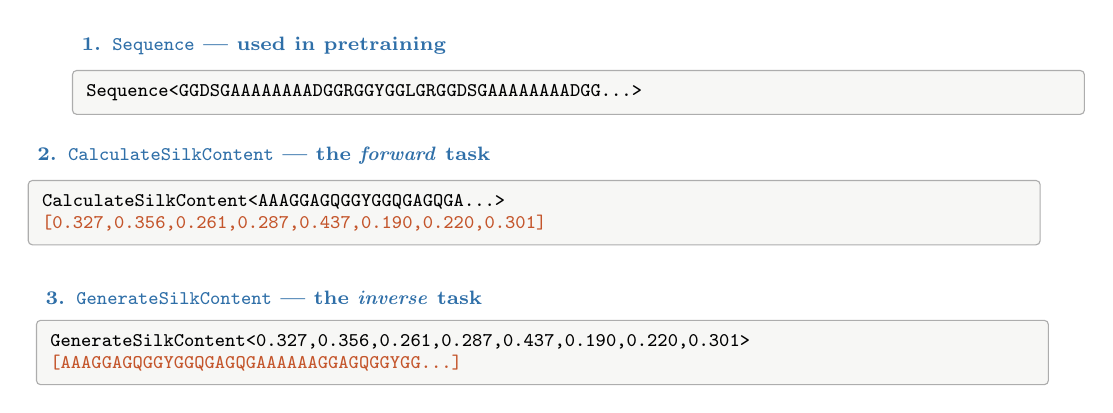
\begin{tikzpicture}[font=\small,
  lab/.style={font=\scriptsize\bfseries,text=papercol},
  tape/.style={draw=greyc!70,fill=codebg,rounded corners=1.5pt,inner sep=5pt,
               font=\ttfamily\scriptsize},
]
\node[lab] (l1) at (0,2.3) {1. \texttt{Sequence} --- used in pretraining};
\node[tape,below=2pt of l1.south west,anchor=north west,text width=12.5cm]
  {Sequence<GGDSGAAAAAAAADGGRGGYGGLGRGGDSGAAAAAAAADGG\ldots>};

\node[lab] (l2) at (0,0.9) {2. \texttt{CalculateSilkContent} --- the \emph{forward} task};
\node[tape,below=2pt of l2.south west,anchor=north west,text width=12.5cm]
  {CalculateSilkContent<AAAGGAGQGGYGGQGAGQGA\ldots>\\
   \textcolor{ourscol}{[0.327,0.356,0.261,0.287,0.437,0.190,0.220,0.301]}};

\node[lab] (l3) at (0,-0.9) {3. \texttt{GenerateSilkContent} --- the \emph{inverse} task};
\node[tape,below=2pt of l3.south west,anchor=north west,text width=12.5cm]
  {GenerateSilkContent<0.327,0.356,0.261,0.287,0.437,0.190,0.220,0.301>\\
   \textcolor{ourscol}{[AAAGGAGQGGYGGQGAGQGAAAAAAGGAGQGGYGG\ldots]}};
\end{tikzpicture}
\caption[The three tasks]{The three fine-tuning formats. Black is the prompt
you supply; orange is what the model generates. The angle brackets hold the
input, the square brackets hold the output. Note that tasks 2 and 3 are the
same information in opposite directions --- that symmetry is what makes the
round trip of Section~\ref{sec:cycle} possible.}
\label{fig:tasks}
\end{figure}

\begin{keybox}{The eight-dimensional property vector}
Equation~(1) of the paper fixes the order, and nothing in the prompt labels the
slots --- the model learned them positionally:
\[
  [\,\underbrace{\text{toughness}}_{0},\;
    \underbrace{\text{SD}}_{1},\;
    \underbrace{E}_{2},\;
    \underbrace{\text{SD}}_{3},\;
    \underbrace{\text{strength}}_{4},\;
    \underbrace{\text{SD}}_{5},\;
    \underbrace{\text{strain}}_{6},\;
    \underbrace{\text{SD}}_{7}\,]
\]
All eight are \term{min--max normalised} to $[0,1]$: for each property, the
minimum and maximum across the dataset are found, and every value is mapped by
\[
  v_{\text{norm}} = \frac{v_{\text{raw}} - \min}{\max - \min}.
\]
Values are always written to three decimal places. Recovering the eight
$(\min,\max)$ pairs, which live in a supplementary table I could not initially
obtain, became one of the more satisfying parts of the project
(Section~\ref{sec:normalisation}).
\end{keybox}

\section{The cycle-consistency procedure}
\label{sec:cycle}

This is the procedure that produces every headline number.

\begin{figure}[htbp]
\centering
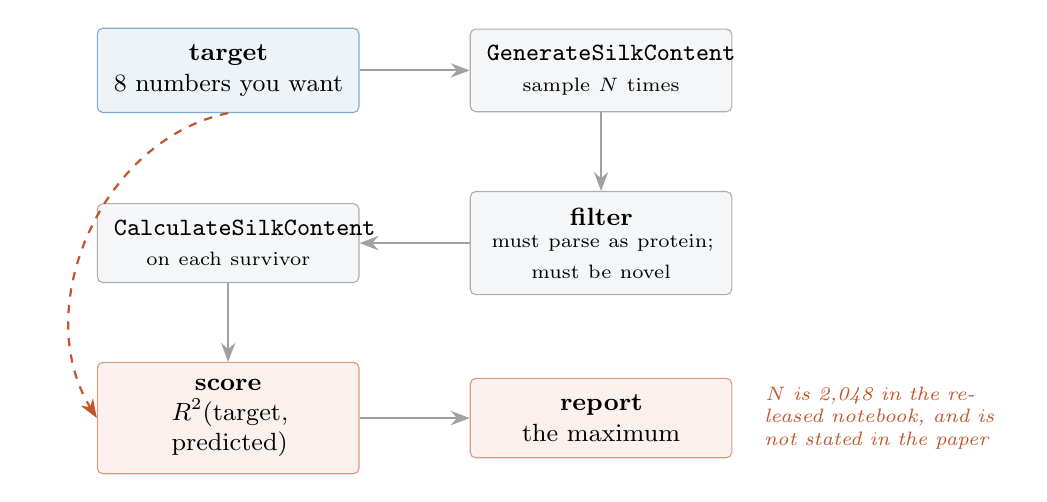
\begin{tikzpicture}[font=\small,
  n/.style={draw=greyc!70,fill=boxbg,rounded corners=2pt,inner sep=6pt,
            text width=2.9cm,align=center,minimum height=1.0cm},
  pn/.style={n,draw=papercol!60,fill=papercol!8},
  on/.style={n,draw=ourscol!60,fill=ourscol!8},
  ar/.style={-{Stealth[length=2.4mm]},thick,greyc!80},
]
\node[pn] (target) {\textbf{target}\\ 8 numbers you want};
\node[n,right=1.4cm of target] (gen) {\texttt{GenerateSilkContent}\\ \scriptsize sample $N$ times};
\node[n,below=1.0cm of gen] (filter) {\textbf{filter}\\ \scriptsize must parse as protein;\\ must be novel};
\node[n,left=1.4cm of filter] (fwd) {\texttt{CalculateSilkContent}\\ \scriptsize on each survivor};
\node[on,below=1.0cm of fwd] (score) {\textbf{score}\\ $R^2$(target, predicted)};
\node[on,right=1.4cm of score] (max) {\textbf{report}\\ the maximum};

\draw[ar] (target) -- (gen);
\draw[ar] (gen) -- (filter);
\draw[ar] (filter) -- (fwd);
\draw[ar] (fwd) -- (score);
\draw[ar] (score) -- (max);
\draw[ar,dashed,ourscol] (target.south) to[bend right=55] (score.west);

\node[right=0.3cm of max,text width=3.1cm,font=\scriptsize\itshape,text=ourscol]
  {$N$ is 2{,}048 in the released notebook, and is not stated in the paper};
\end{tikzpicture}
\caption[The cycle]{The cycle-consistency loop. A target goes in, $N$
candidate sequences come out, each is fed back through the forward task, and
the best-scoring one is reported. The dashed line is where the \Rsq{} of
Section~\ref{sec:r2trap} is computed --- \emph{within} one eight-vector.}
\label{fig:cycle}
\end{figure}

Written out:

\begin{enumerate}[leftmargin=*,itemsep=2pt]
  \item Choose an 8-vector target $\mathbf{t}$.
  \item Sample $N$ sequences from \code{GenerateSilkContent<$\mathbf{t}$>}.
  \item Discard any that do not parse as a protein.
  \item Discard any that exactly match a known silk sequence --- this is the
        paper's definition of \term{novel}.
  \item For each survivor $s$, compute $\mathbf{p} =
        \code{CalculateSilkContent}(s)$.
  \item Score $R^2(\mathbf{t}, \mathbf{p})$ across the eight entries.
  \item Report $\max$ over all survivors.
\end{enumerate}

\section{The eight property targets}

The paper picks eight targets. Three are described as random, for assessing
forward prediction (Figure 3 of the paper). Five are chosen deliberately to
span common, rare, and physically non-existent combinations (Figures 4--7).

\begin{table}[htbp]
\centering
\small
\caption[The eight targets]{The eight target vectors and the \Rsq{} the paper
reports for each. I use the labels F1--F3 and S1--S5 throughout; the paper
numbers them 1--3 and 1--5.}
\label{tab:targets}
\begin{tabular}{llcl}
\toprule
\textbf{ID} & \textbf{8-vector} & \textbf{paper \Rsq} & \textbf{rationale} \\
\midrule
F1 & [0.600, 0.204, 0.279, 0.043, 0.329, 0.127, 0.502, 0.139] & 0.8764 & random \\
F2 & [0.300, 0.200, 0.200, 0.100, 0.300, 0.100, 0.200, 0.100] & 0.8369 & random \\
F3 & [0.100, 0.200, 0.200, 0.040, 0.300, 0.100, 0.700, 0.100] & 0.6889 & random \\
\midrule
S1 & [0.250, 0.252, 0.200, 0.151, 0.310, 0.203, 0.293, 0.265] & 0.8899 & common $(E,T)$ pair \\
S2 & [0.550, 0.252, 0.750, 0.151, 0.310, 0.203, 0.293, 0.265] & 0.5640 & rare, high $E$ \\
S3 & [1.000, 0.252, 0.450, 0.151, 0.200, 0.203, 0.293, 0.265] & 0.7167 & rare, high toughness \\
S4 & [0.900, 0.252, 0.800, 0.151, 0.310, 0.203, 0.293, 0.265] & 0.7843 & \emph{non-existent} pair \\
S5 & [0.240, 0.252, 0.206, 0.151, 0.270, 0.203, 0.293, 0.265] & 0.7751 & common (strength, $T$) \\
\bottomrule
\end{tabular}
\end{table}

S4 is the interesting one scientifically: high toughness \emph{and} high
stiffness together, a combination that does not occur in the 1{,}033 measured
silks. Asking the model for it is asking for a material better than anything
nature produced. That the model returns \emph{something} is the paper's
headline capability claim.

\begin{warnbox}{An internal inconsistency worth noting}
The paper says that for each of S1--S5, the properties not being varied are set
to dataset \emph{medians}. Sets S1, S2 and S4 all carry strength $= 0.310$. Set
S3 varies toughness and $E$, so its strength should also be $0.310$ --- but both
Table~1 and the Figure~2 caption give $\mathbf{0.200}$.

Two independent places in the paper agree with each other, so this is not a
typesetting slip in one location. I kept the published value, because changing
a published input to get a better match is not reproduction. It does change
S3's target spread and therefore its \Rsq{}. Recorded as discrepancy D2.
\end{warnbox}

\section{What the paper's figures show}

Since I refer to these repeatedly, here is what each one is.

\begin{description}[leftmargin=0cm,style=nextline,itemsep=5pt]

\item[Figure 2 --- the property landscape.] A pair plot of the 1{,}033
  normalised property values: histograms on the diagonal, scatter below,
  density contours above. It establishes the distributions are roughly uniform,
  that toughness and strength are positively correlated, and it marks the five
  chosen targets in red so you can see which are common and which are out on
  the edge.

\item[Figure 3 --- forward prediction, three targets.] Bar charts. For each of
  F1--F3, eight blue bars (requested) beside eight red bars (predicted). Visual
  agreement, quantified by the \Rsq{} above each panel.

\item[Figure 4 --- the same for the five selected targets.] Same format,
  S1--S5. This is where 0.8899, 0.5640, 0.7167, 0.7843 and 0.7751 come from.

\item[Figure 5 --- do the designs look like real proteins?] For each generated
  sequence and its two closest database relatives: sequence length, molecular
  weight, instability index, isoelectric point, amino-acid composition, and
  secondary-structure fractions. The argument is that the generated sequences
  sit in the same range as natural ones.

\item[Figure 6 --- folded structures.] AlphaFold2 predictions for five
  generated sequences and one natural relative each. The paper is careful here:
  confidence scores (pLDDT) are 40--60, which is low, and it limits the claim to
  visual comparison. I did not attempt this.

\item[Figure 7 --- motifs.] Counts of specific short sequence motifs in the
  generated sequences versus their natural relatives, plus density plots of
  \emph{where} along the sequence each motif sits. The motif definitions come
  from a supplementary table which in turn derives from the Silkome paper.

\end{description}

\begin{keybox}{The one about secondary structure, which I have to flag now}
Figure 5 reports ``secondary structure fraction'', defined in its caption as
the proportion of residues that tend to be in
\begin{center}
helix (\aaseq{V I Y F W L}), \quad turn (\aaseq{N P G S}), \quad sheet (\aaseq{E M A L}).
\end{center}
Those groupings are exactly what Biopython's
\code{secondary\_structure\_fraction()} used up to version~1.81, and the caption
reproduces that function's own documentation of the time.

Biopython v1.82 changed the method, and its current docstring says why:
prior to 1.82 it \emph{``wrongly returned (Sheet, Turn, Helix) while claiming to
return (Helix, Turn, Sheet)''}. The set \aaseq{V I Y F W L} is a \emph{sheet}
propensity set; \aaseq{E M A L} is a \emph{helix} set.

So under the corrected assignment the labels in Figure 5c are exchanged. The
paper used the library as documented when it was written; the correction is
upstream and postdates publication. It matters more here than it would
elsewhere, because $\beta$-sheet content is \emph{the} central structural
quantity in spider silk (Chapter~\ref{ch:biology}), so a reader comparing
Figure 5c against the silk literature would draw the wrong conclusion about
which residues drive sheet formation. My code computes both conventions and
reports both. Recorded as discrepancy D1.
\end{keybox}

\section{What the paper claims, stated fairly}

It is worth writing down precisely what is and is not being asserted, because
much of my later analysis is about the gap between the two.

\textbf{The paper does claim:}
\begin{itemize}[leftmargin=*,itemsep=1pt]
  \item A model that generates novel spidroin sequences to order.
  \item Self-consistency between its forward and inverse directions, quantified
        by \Rsq.
  \item That generated sequences resemble natural ones on standard descriptors
        and motif content.
  \item That property combinations absent from nature can be requested and
        something is returned.
\end{itemize}

\textbf{The paper does not claim:}
\begin{itemize}[leftmargin=*,itemsep=1pt]
  \item Held-out predictive accuracy. It says plainly that fine-tuning used all
        known pairs.
  \item That the generated sequences would actually have those properties if
        synthesised. Its own limitations section says validation would require
        molecular dynamics or wet-lab work.
\end{itemize}

\begin{keybox}{The gap I set out to measure}
Both lists are accurate. But a reader encountering ``\Rsq{} $= 0.89$'' in a
property-prediction context will, by default, read it as the \emph{first} list
plus a bit of the second. The number is a maximum over an unstated $N$, of a
within-vector self-consistency measure, from a model that saw all its data.
Each of those three qualifiers is individually reasonable; together they mean
the number measures something much narrower than it appears to.

Nothing about that is misconduct or error. It is under-specification, and it is
extremely common. Measuring how much each qualifier is worth is what the four
extensions do.
\end{keybox}

\chapter{The reproduction}
\label{ch:reproduction}

\section{What "reproduce" means here, and the hardware}

There are degrees of reproduction. From weakest to strongest:

\begin{enumerate}[leftmargin=*,itemsep=2pt]
  \item Re-run the authors' notebook unchanged.
  \item Re-implement the analysis from the paper, using their released model.
  \item Retrain the model from scratch and re-derive everything.
\end{enumerate}

This project is a thorough version of (2). I rebuilt the data pipeline,
the metrics and the analysis from the paper's description and primary sources,
and used the released checkpoint. I did not retrain --- pretraining on 600{,}000
proteins is well beyond a laptop.

Hardware: an NVIDIA RTX 4050 laptop GPU with 6\,GB of memory. The model is
253.6M parameters, which at half precision is about 0.5\,GB --- comfortable for
inference. Total compute for everything in these notes was roughly six
GPU-hours.

\begin{keybox}{The discipline I held to}
Every choice the paper does not specify is written down as a numbered
assumption (A1--A15) with its reasoning and, where possible, evidence. Every
place my result differs from the paper's, or where the paper is internally
inconsistent, is a numbered discrepancy (D1--D15) stated neutrally. Every script
writes a JSON manifest recording the git commit, the model revision, the random
seed, the platform and the version of every library. No number in these notes
exists without a file behind it.
\end{keybox}

\section{Step 1: is the released model the model described?}
\label{sec:checkpoint}

Before anything else: does the checkpoint on Hugging Face match the paper?

\begin{table}[htbp]
\centering\small
\caption{Architecture check. \code{scripts/00\_check\_env.py}.}
\begin{tabular}{lcc}
\toprule
& \textbf{paper} & \textbf{checkpoint} \\
\midrule
layers & 12 & 12 \\
attention heads & 8 & 8 \\
hidden size & 1024 & 1024 \\
feed-forward size & 4096 & 4096 \\
parameters & 253.6\,M & \textbf{253{,}556{,}736} \\
architecture & GPT-NeoX-style & \code{gpt\_neox} \\
\bottomrule
\end{tabular}
\end{table}

All four stated hyperparameters match and the parameter count agrees to the
paper's rounding. The resolved commit hash is recorded so a future run uses
identical weights.

\subsection{The sharpest test available}

Architecture matching is necessary but weak --- it says nothing about the
weights. Something stronger was needed: a test with a \emph{known correct
answer}.

The paper's Experimental Section prints one fine-tuning record in full: a
sequence, and the eight values paired with it. If this really is the fine-tuned
model, feeding it that sequence should return that vector.

\begin{goodbox}{It does, exactly}
\begin{center}
\code{[0.327, 0.356, 0.261, 0.287, 0.437, 0.190, 0.220, 0.301]}
\end{center}
All eight entries, matching the published vector. This exercises the tokenizer,
the prompt format, the weights and my output parser in one shot, and unlike
every other test in the project it has an externally known answer.
\end{goodbox}

There is a wrinkle here that I initially got wrong, and which turned out to be
in my favour --- it is discrepancy D8 and I tell that story in
Section~\ref{sec:d8}.

\section{Step 2: rebuilding the 1{,}033-pair dataset}
\label{sec:dataset}

The paper says its dataset was ``constructed and curated based on the silkome
dataset'' and contains 1{,}033 pairs. It does not say how. The pairs are not in
the authors' repository. So they had to be rebuilt from the Silkome release.

My first attempt joined the two Silkome files on \code{ncbi\_tax\_id}, the
species identifier present in both. It returned \textbf{zero rows}. The field
exists in both files but shares no values --- they are different numbering
schemes.

The correct key is \code{idv\_id}: the individual spider.

\begin{figure}[htbp]
\centering
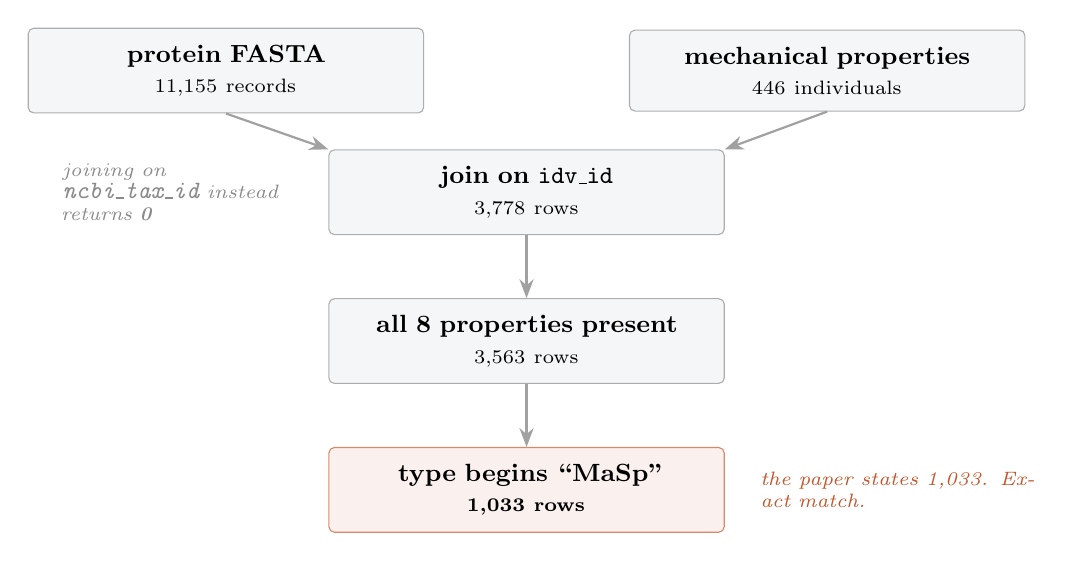
\begin{tikzpicture}[font=\small,
  b/.style={draw=greyc!70,fill=boxbg,rounded corners=2pt,inner sep=6pt,
            text width=4.6cm,align=center},
  ar/.style={-{Stealth[length=2.4mm]},thick,greyc!80},
  num/.style={font=\scriptsize\bfseries,text=ourscol},
]
\node[b] (fasta) {\textbf{protein FASTA}\\ \scriptsize 11{,}155 records};
\node[b,right=2.6cm of fasta] (mech) {\textbf{mechanical properties}\\ \scriptsize 446 individuals};
\node[b,below=1.0cm of $(fasta)!0.5!(mech)$] (join) {\textbf{join on \code{idv\_id}}\\ \scriptsize 3{,}778 rows};
\node[b,below=0.8cm of join] (comp) {\textbf{all 8 properties present}\\ \scriptsize 3{,}563 rows};
\node[b,below=0.8cm of comp,draw=ourscol!70,fill=ourscol!8] (masp)
  {\textbf{type begins ``MaSp''}\\ \scriptsize \textbf{1{,}033 rows}};

\draw[ar] (fasta.south) -- (join.north west);
\draw[ar] (mech.south) -- (join.north east);
\draw[ar] (join) -- (comp);
\draw[ar] (comp) -- (masp);

\node[right=0.35cm of masp,text width=3.6cm,font=\scriptsize\itshape,text=ourscol]
  {the paper states 1{,}033. Exact match.};
\node[left=0.35cm of join,text width=2.9cm,font=\scriptsize\itshape,text=greyc]
  {joining on \code{ncbi\_tax\_id} instead returns \textbf{0}};
\end{tikzpicture}
\caption[Dataset reconstruction]{Rebuilding the fine-tuning set. The rule was
found by searching for one that lands on the published count; hitting 1{,}033
exactly is strong evidence it is the authors' rule, though it remains a
reconstruction (assumption A1).}
\label{fig:dataset}
\end{figure}

Three properties of the result are worth knowing:

\begin{itemize}[leftmargin=*,itemsep=3pt]
  \item \textbf{1{,}033 rows but 1{,}028 distinct sequences.} Five sequences
        appear twice with \emph{different} property values, because the same
        protein was recovered from two individuals whose fibres tested
        differently. So the dataset contains contradictory labels for five
        inputs. I kept both, since the published count requires it (A12).
  \item \textbf{553 CTD, 480 NTD.} Terminal-domain-anchored records, as
        discussed in Section~\ref{sec:silkome}.
  \item Lengths run 115--1854, median 378. Types: MaSp1 349, MaSp2 331,
        MaSp 223, MaSp3B 47, MaSp3 43, MaSp2B 40.
\end{itemize}

\section{Step 3: recovering the normalisation constants}
\label{sec:normalisation}

To convert raw measurements into the model's $[0,1]$ scale you need the eight
$(\min, \max)$ pairs. They live in the paper's Table S5, in Supporting
Information that --- at this stage of the project --- I could not obtain.

So I derived them. The Experimental Section gives one clue: the extremes were
taken ``across the entire dataset (not limited to MaSp sequences)''. That
sentence has at least three readings, so I tested all three against the one
published normalised vector I had, from the worked example.

\begin{table}[htbp]
\centering\small
\caption[Normalisation candidates]{Testing three readings of ``the entire
dataset'' against the paper's own published vector.}
\begin{tabular}{lc}
\toprule
\textbf{population used for min/max} & \textbf{max abs.\ error vs published} \\
\midrule
raw \code{mechanical\_properties.csv} (446 rows) & 0.139 \\
\textbf{sequence-joined, all spidroin types (3{,}563 rows)} & \textbf{0.00047} \\
sequence-joined, MaSp only (1{,}033 rows) & 0.054 \\
\bottomrule
\end{tabular}
\end{table}

The middle reading reproduces all eight published values to within the paper's
own three-decimal rounding.

\begin{goodbox}{Later confirmed outright}
Much later I located the Supporting Information appended to the arXiv preprint
of the same paper. Table~S5 is there, with units. Every one of my recovered
constants matches:

\begin{center}
\small
\begin{tabular}{lccc}
\toprule
property & unit & Table~S5 & recovered \\
\midrule
toughness & GJ/m$^3$ & 0.005 -- 0.39 & 0.005 -- 0.39 \\
SD toughness & GJ/m$^3$ & 0.001 -- 0.136 & 0.001 -- 0.136 \\
$E$ & GPa & 0.38 -- 37.0 & 0.38 -- 37.0 \\
SD $E$ & GPa & 0.03 -- 9.76 & 0.03 -- 9.76 \\
strength & GPa & 0.17 -- 3.33 & 0.17 -- 3.33 \\
SD strength & GPa & 0.01 -- 0.8 & 0.01 -- 0.8 \\
strain & \% & 5.1 -- 53.2 & 5.1 -- 53.2 \\
SD strain & \% & 0.1 -- 13.7 & 0.1 -- 13.7 \\
\bottomrule
\end{tabular}
\end{center}

This also confirms the dataset reconstruction from a second direction: the
constants are a property of the population they were computed over, so getting
them exactly right means I assembled the same population the authors did.
\end{goodbox}

\section{Step 4: a decoding decision, and why it needed measuring}
\label{sec:decodingchoice}

The released notebook decodes the forward task by \emph{sampling} at
temperature 0.01. I decode \emph{greedily}. That is a deliberate departure, and
since departures need justifying, I measured the consequences on 60 real silk
sequences.

\begin{table}[htbp]
\centering\small
\caption[Decoding diagnostics]{\code{scripts/01b\_forward\_decoding\_diagnostics.py}}
\begin{tabular}{lc}
\toprule
\textbf{question} & \textbf{answer} \\
\midrule
Do greedy and sampled agree? & identical on \textbf{58/60} (96.7\%) \\
Where they differ, by how much? & at most 0.38 in one slot, 2 sequences \\
Does greedy parse at the 64-token budget? & \textbf{60/60} \\
Does 32 tokens suffice? & \textbf{0/60} --- the answer is cut off \\
Is greedy invariant to batch size? & \textbf{16/16} identical \\
Is sampled invariant to batch size? & \textbf{no} \\
\bottomrule
\end{tabular}
\end{table}

The last row is the reason. I batch the forward pass for speed, and all rows of
a batch draw from one random number stream. Under sampling, a candidate's
predicted properties would depend on \emph{which other candidates happened to
share its batch} --- a reproducibility disaster that is entirely mine to solve,
since the authors did not batch.

There was also an incidental discovery: under sampling, the model sometimes
continues the amino-acid sequence \emph{before} emitting the property vector,
and can then be cut off mid-answer by the 64-token budget. The released
notebook catches that in a bare \code{except:}, so those cases silently vanish.
Under greedy decoding it never happens.

\begin{warnbox}{This choice was later exonerated}
A reader could reasonably worry that greedy decoding is why my numbers came out
lower than the paper's. I tested exactly that in
Section~\ref{sec:stochasticity} and the effect is $+0.0065$ --- two orders of
magnitude too small. Recorded as assumption A5.
\end{warnbox}

\section{Step 5: re-running the whole procedure}
\label{sec:table1}

With everything rebuilt, I ran the cycle-consistency procedure of
Figure~\ref{fig:cycle} for all eight targets, with $N = 2048$ generation
attempts each, matching the notebook's budget. About 4.5 GPU-hours.

\begin{table}[htbp]
\centering\small
\caption[Table 1 reproduction]{The headline reproduction. ``Pool'' is the
number of candidates that parsed \emph{and} were novel, and so could be scored.}
\label{tab:repro}
\begin{tabular}{lccccc}
\toprule
\textbf{set} & \textbf{paper \Rsq} & \textbf{our max} & \textbf{our mean} & \textbf{our median} & \textbf{pool} \\
\midrule
F1 & 0.8764 & 0.7221 & $-0.36$ & $-0.03$ & 815 \\
F2 & 0.8369 & 0.6964 & $-3.57$ & $-1.41$ & 739 \\
F3 & 0.6889 & \textbf{0.6780} & $-0.36$ & $+0.09$ & 735 \\
S1 & 0.8899 & 0.7120 & $-6.54$ & $-2.25$ & 712 \\
S2 & 0.5640 & 0.2234 & $-0.71$ & $-0.67$ & 738 \\
S3 & 0.7167 & 0.6494 & $-0.37$ & $-0.31$ & 752 \\
S4 & 0.7843 & 0.3487 & $-0.49$ & $-0.48$ & 710 \\
S5 & 0.7751 & 0.6233 & $-11.59$ & $-3.61$ & 641 \\
\bottomrule
\end{tabular}
\end{table}

\begin{warnbox}{Partial reproduction}
I do not reach the published value on \emph{any} of the eight sets. The gap
runs from 0.011 (F3, essentially reproduced) to 0.436 (S4), mean 0.27.
Across all eight, none of roughly 700--800 candidates matched or exceeded the
published figure.

The mechanism works --- the pipeline does produce sequences whose predicted
properties approach the request --- but the magnitude I obtain is lower. That is
a partial reproduction and I describe it as one.
\end{warnbox}

Two things in this table deserve attention beyond the gap.

\paragraph{The mean and median are terrible.} For six of eight sets, the
\emph{typical} candidate has negative \Rsq{} --- worse than guessing the average.
S5's mean is $-11.59$. The maximum is doing enormous work.

\paragraph{The pool is much smaller than the budget.} 2{,}048 attempts yield
only $\sim$700--800 scoreable candidates. Where did the rest go? About 5\% fail
to parse. The rest --- the large majority of the loss --- were discarded for not
being novel. That deserves its own measurement, in
Section~\ref{sec:regurgitation}.

\subsection{Testing one explanation for the gap}
\label{sec:stochasticity}

Before attributing the shortfall to anything, one purely statistical mechanism
had to be ruled out.

The notebook scores candidates with a \emph{sampled} forward pass. So each
candidate's \Rsq{} is itself a random variable, and a maximum over $N$ noisy
scores is inflated relative to a maximum over $N$ noiseless ones --- roughly by
the scale of the scoring noise. My scores are noiseless. Could that alone
explain 0.27?

I re-scored the \emph{identical} candidate sequences with the notebook's
sampled decoder --- same sequences, same targets, only the scorer changed.

\begin{table}[htbp]
\centering\small
\caption[Scoring stochasticity]{\code{scripts/10b\_scoring\_stochasticity.py}}
\begin{tabular}{lcccc}
\toprule
\textbf{set} & \textbf{max, greedy} & \textbf{max, sampled} & \textbf{inflation} & \textbf{gap remaining} \\
\midrule
S1 & 0.7120 & 0.7379 & $+0.026$ & 0.152 \\
F1 & 0.7221 & 0.7221 & $0.000$ & 0.154 \\
S4 & 0.3487 & 0.3487 & $0.000$ & 0.436 \\
S2 & 0.2234 & 0.2234 & $0.000$ & 0.341 \\
\bottomrule
\end{tabular}
\end{table}

Mean inflation $+0.0065$; scores identical on 97--99\% of candidates. The
hypothesis is \textbf{rejected}. At this point in the project I recorded the gap
as unexplained rather than attributing it to anything --- which was the right
call, because the answer arrived later and from an unexpected direction.

\section{Step 6: the answer, once the Supporting Information turned up}
\label{sec:exactmatch}

Late in the project I found the supplementary tables appended to the arXiv
preprint of the same paper (\code{arXiv:2309.10170}, pages 31--38). Wiley's copy
refuses automated requests, but arXiv does not.

Table~S1 lists the five sequences the paper actually generated. Table~S3 lists,
for each, the property vector its forward task predicted and the resulting
\Rsq. So both the input and the expected output are known, and the scorer can
be tested with no sampling and no search at all.

Extracting those sequences correctly took two attempts and is the subject of
Section~\ref{sec:tables1}. With them verified:

\begin{goodbox}{The forward task reproduces exactly}
\begin{center}
\small
\begin{tabular}{lccc}
\toprule
\textbf{set} & \textbf{paper \Rsq} & \textbf{ours} & \textbf{predicted vector vs Table S3} \\
\midrule
S1 & 0.8899 & \textbf{0.8899} & \textbf{8/8 slots identical} \\
S2 & 0.5640 & 0.5176 & 6/8 \\
S3 & 0.7167 & \textbf{0.7167} & \textbf{8/8} \\
S4 & 0.7843 & \textbf{0.7843} & \textbf{8/8} \\
S5 & 0.7751 & \textbf{0.7751} & \textbf{8/8} \\
\bottomrule
\end{tabular}
\end{center}

Four of five reproduce to four decimal places --- and not merely in \Rsq, but in
the entire eight-value predicted vector, slot for slot. S2 agrees on its first
six slots and differs on the last two, consistent with the paper's sampled
decoding diverging from greedy on a low-confidence tail.
\end{goodbox}

\begin{keybox}{What this settles}
The checkpoint, the prompt format, the parser, the normalisation and my
decoding choice are all \emph{exonerated}. Given the paper's own sequences, the
scorer returns the paper's own answers.

So the shortfall in Section~\ref{sec:table1} is located precisely: it is in the
\textbf{inverse task's search}. My 2{,}048 candidates simply did not contain
sequences as good as the ones the authors found. Their generated sequences are
also markedly longer --- 1096, 926, 312, 869 and 521 residues against my 530,
493, 471, 185 and 256 --- so the two searches explored different regions of the
space. Why theirs found longer and better candidates, I cannot say from the
information available.

This is a considerably stronger reproduction result than
Section~\ref{sec:table1} suggests on its own, and it is why these notes present
the two together.
\end{keybox}

\subsection{Figure 7, against the paper's own specimens}

With Table~S1 in hand, the motif analysis could finally be run the way the
paper ran it: each generated sequence against \emph{its own} two BLAST
relatives, using the Table~S4 motif definitions.

\begin{center}
\small
\begin{tabular}{lcl}
\toprule
\textbf{set} & \textbf{motif-density correlation} & \textbf{the paper's wording} \\
\midrule
S1 & 0.658 & ``particularly evident'' \\
S2 & \textbf{0.448} & ``congruence is diminished in set 2'' \\
S3 & \textbf{0.941} & ``particularly evident'' \\
S4 & \textbf{0.944} & ``particularly evident'' \\
S5 & 0.660 & --- \\
\bottomrule
\end{tabular}
\end{center}

This supports the paper's qualitative claim: set 2 is the weakest by a clear
margin, exactly as reported, and sets 3 and 4 are strongest. Set 1, which the
paper groups with 3 and 4, comes out middling here.

\begin{warnbox}{A lesson about substitutes}
Before I had Table~S1, I ran the same analysis using \emph{nearest database
neighbours} as stand-ins for the BLAST relatives. That version gave S2 $= 0.99$
and S4 $= -0.02$ --- close to the reverse of the correct ordering.

A reproduction that had stopped at the substitute specimens would have reported
something wrong, with no internal sign of trouble. Substituting one input for
another is sometimes unavoidable, but the substitution is a claim in its own
right and deserves the same scrutiny as the result.
\end{warnbox}

\subsection{Descriptors, checked against the paper's own numbers}

Table~S3 also publishes molecular weight, instability index and isoelectric
point for all fifteen sequences. Recomputing them is an independent check of
the Figure 5 pipeline:

\begin{center}
\small
\begin{tabular}{lc}
\toprule
molecular weight & \textbf{15/15} match \\
isoelectric point & \textbf{15/15} match \\
instability index & 13/15 match \\
\bottomrule
\end{tabular}
\end{center}

The two instability-index misses are both explained. Two sequences contain
\aaseq{X} --- an ``unknown residue'' code that appears in real database records.
Biopython refuses to weigh a sequence containing \aaseq{X}, yet the paper
reports a weight. Recovering the implied mass,
\[
  \frac{\text{published MW} - \text{MW with \aaseq{X} dropped}}{\text{number of \aaseq{X}}}
  = 111.985 \text{ Da}
\]
for both sequences independently --- the conventional average residue mass. So
the paper's tool weighed unknowns as average residues. Applying that convention
reproduces both weights exactly. The instability index still differs slightly
(28.88 vs 28.55) because that index is computed from \emph{dipeptides}, and
removing an \aaseq{X} joins its two neighbours into a pair that was never in the
sequence. A consequence of the unknown-residue handling, not a disagreement
about the sequence --- reported rather than tuned away.

\chapter{The four extensions}
\label{ch:extensions}

Reproducing a result tells you whether it holds. It does not tell you what it
measures. These four experiments ask that question, and they converge on a
single answer.

\section{Extension 1: how much of the number is the search?}
\label{sec:bestofn}

Section~\ref{sec:bestofn-concept} set out the idea; here is the measurement.
Every candidate generated in Section~\ref{sec:table1} was kept, so the full
distribution of \Rsq{} is available, not just its maximum.

\begin{figure}[htbp]
\centering
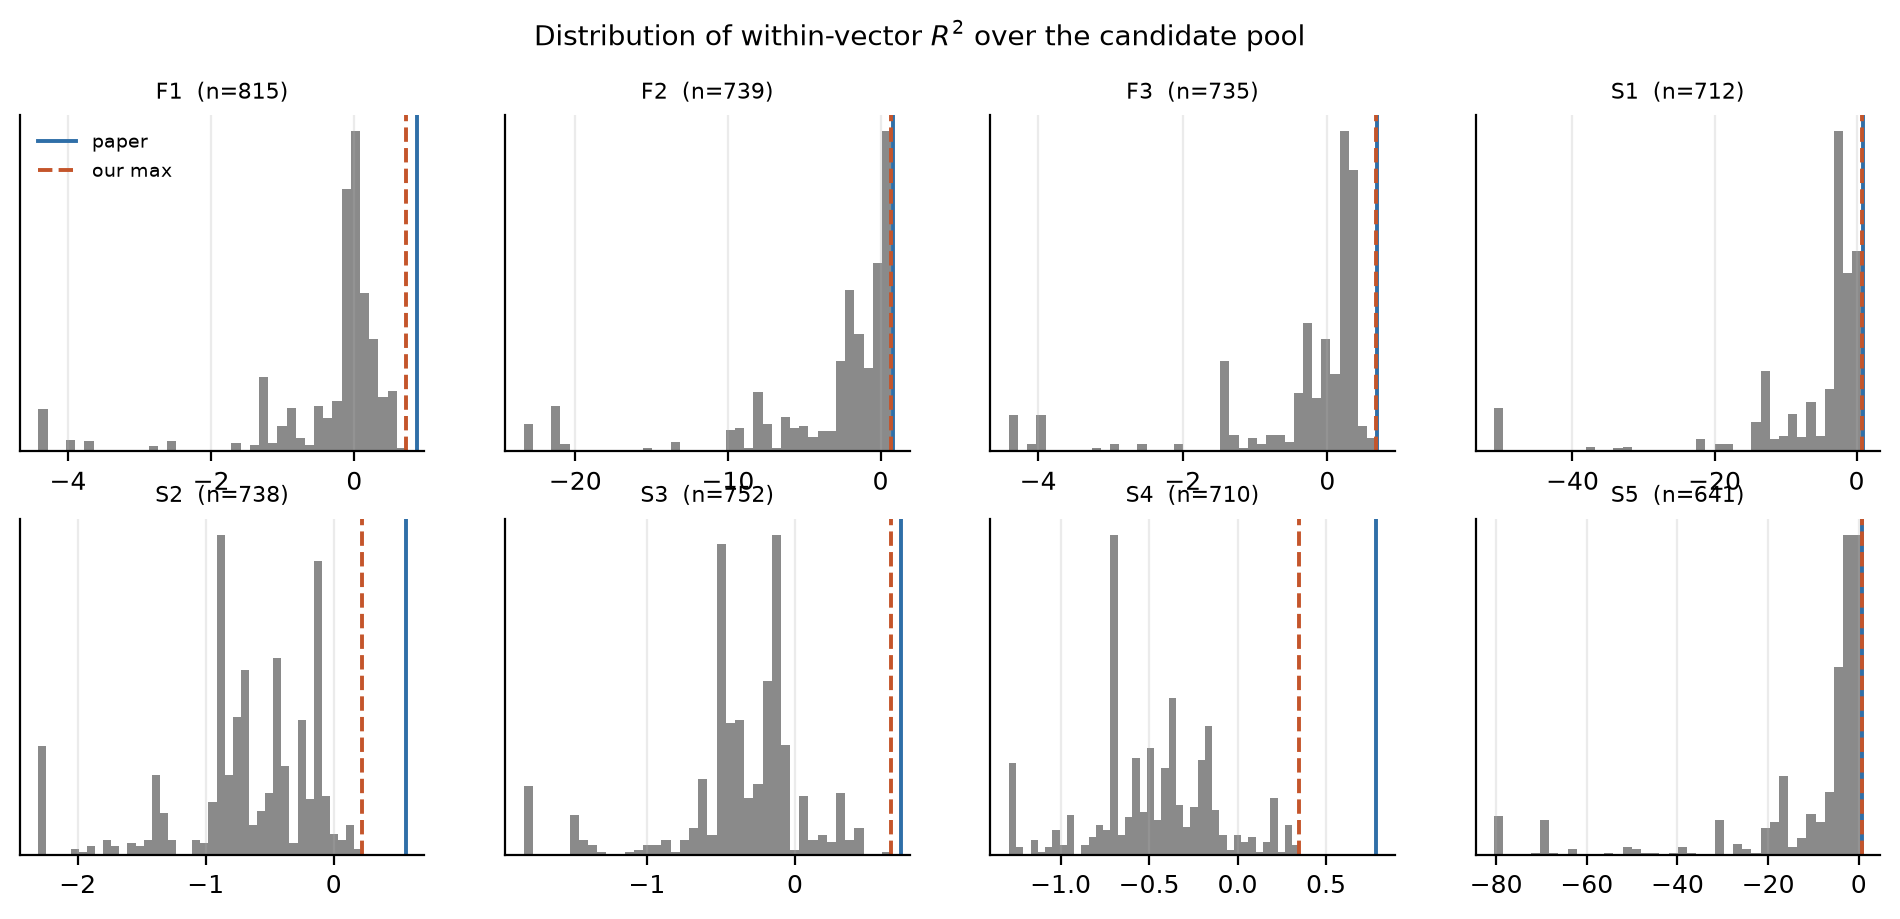
\includegraphics[width=\linewidth]{figures/fig3_r2_distribution.png}
\caption[R-squared distributions]{\textbf{The distribution the paper reports the
maximum of.} One panel per target; each histogram is the \Rsq{} of $\sim$700--800
individually generated candidates. The blue line is the paper's published
value, the dashed orange line is my pool maximum. Two things to see. First, the
mass of the distribution sits at or below zero --- the typical candidate is
worse than guessing the mean. Second, both vertical lines are far out in the
right tail, which is the visual statement of the whole best-of-$N$ argument.
The left tails are clipped at the 2nd percentile; they run to $-100$ and beyond
for some sets, which is why the means in Table~\ref{tab:repro} look extreme.}
\label{fig:r2dist}
\end{figure}

Bootstrapping from each pool gives the expected best score as a function of the
budget:

\begin{table}[htbp]
\centering\small
\caption[Best-of-N curves]{Expected best \Rsq{} after $N$ draws. Capped at
$N \le$ pool$/10$; beyond that the bootstrap is really just reporting the pool
maximum back, not estimating anything independent of it.}
\label{tab:bestofn}
\begin{tabular}{lccccccc}
\toprule
\textbf{set} & $N{=}1$ & $2$ & $4$ & $8$ & $16$ & $32$ & $64$ \\
\midrule
F1 & $-0.36$ & $+0.06$ & 0.23 & 0.34 & 0.44 & 0.51 & 0.56 \\
F2 & $-3.40$ & $-0.86$ & 0.05 & 0.40 & 0.54 & 0.58 & 0.59 \\
F3 & $-0.34$ & $+0.13$ & 0.30 & 0.37 & 0.42 & 0.47 & 0.54 \\
S1 & $-6.49$ & $-2.09$ & $-0.66$ & $-0.07$ & 0.26 & 0.44 & 0.55 \\
S2 & $-0.70$ & $-0.38$ & $-0.22$ & $-0.09$ & $-0.02$ & 0.03 & 0.09 \\
S3 & $-0.36$ & $-0.15$ & $+0.01$ & 0.12 & 0.25 & 0.35 & 0.42 \\
S4 & $-0.48$ & $-0.28$ & $-0.10$ & $+0.01$ & 0.14 & 0.23 & 0.28 \\
S5 & $-11.71$ & $-3.43$ & $-1.29$ & $-0.45$ & $-0.03$ & 0.21 & 0.34 \\
\bottomrule
\end{tabular}
\end{table}

\begin{figure}[htbp]
\centering

\includegraphics[width=0.92\linewidth]{figures/fig2_bestofn.png}
\caption[Best-of-N curves plotted]{\textbf{The same data as a curve.} Horizontal
axis is the sampling budget on a log scale; vertical axis is the expected best
\Rsq. Each colour is one target; dotted horizontal lines are the paper's
published values; shaded bands are 5th--95th percentiles over bootstrap
replicates. Every curve climbs steeply and monotonically. Nothing about the
model changes along these curves --- only how many times you ask it. The axis is
clipped at $-2$ because three sets have $N{=}1$ means below that.}
\label{fig:bestofn}
\end{figure}

\begin{goodbox}{Result}
A single draw from the inverse task is typically worse than useless: the median
candidate has negative \Rsq{} in six of eight sets. Essentially all of the
apparent performance is produced by generating many candidates and keeping the
best.
\end{goodbox}

\begin{keybox}{What does \emph{not} follow}
This is not a criticism of the method. Screening thousands of cheap candidates
is exactly the right procedure when generation costs nothing and evaluation
costs less. If you can make 2{,}000 designs and test them in silico, take the
best one --- obviously.

The objection is narrower, and it is about reporting. Given only the maximum, a
reader cannot tell how much search produced it, cannot compare it against
another method's single-shot number, and cannot estimate the compute needed to
match it. Stating $N$, or showing this curve, costs nothing and removes the
ambiguity entirely.
\end{keybox}

\section{Extension 2: what does the model read from the sequence?}
\label{sec:ablations}

If the forward task computes properties from sequence features, then editing
those features should move the prediction in interpretable ways. This
experiment does controlled surgery on 30 real MaSp sequences and measures how
far the prediction moves.

\subsection{Getting the reference points right}

Two things had to be established before any effect could be interpreted.

\paragraph{A floor.} How much does the prediction move when nothing
meaningful changes? The obvious answer --- resubmit the identical prompt --- gives
exactly zero under greedy decoding, by construction. That floor can never
reject anything, so it is useless as a safeguard. I therefore added a real one:
a \term{conservative point mutation}, one residue swapped for a chemically
similar one, the smallest edit that changes the sequence at all. Measured at
\textbf{0.0148}, with a median of exactly zero --- most single substitutions
change nothing.

\paragraph{A scale.} A shift of ``0.13'' means nothing without knowing the
range. Across 30 unmodified natural sequences, the model's output varies by
\textbf{0.0874}. Every effect below is quoted as a multiple of that.

\subsection{The edits}

\begin{figure}[htbp]
\centering
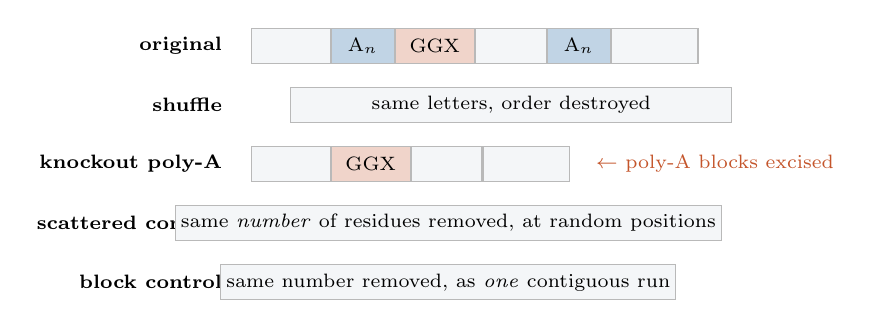
\begin{tikzpicture}[font=\scriptsize,
  seq/.style={draw=greyc!60,minimum height=0.45cm,inner sep=2pt},
  pa/.style={seq,fill=papercol!30},
  gg/.style={seq,fill=ourscol!25},
  o/.style={seq,fill=boxbg},
  lbl/.style={font=\scriptsize\bfseries,anchor=east},
]
% original
\node[lbl] at (-0.25,0) {original};
\node[o,minimum width=1.0cm] (a1) at (0.5,0) {};
\node[pa,minimum width=0.8cm,right=0pt of a1] (a2) {A$_n$};
\node[gg,minimum width=1.0cm,right=0pt of a2] (a3) {GGX};
\node[o,minimum width=0.9cm,right=0pt of a3] (a4) {};
\node[pa,minimum width=0.8cm,right=0pt of a4] (a5) {A$_n$};
\node[o,minimum width=1.1cm,right=0pt of a5] (a6) {};

% shuffle
\node[lbl] at (-0.25,-0.75) {shuffle};
\node[o,minimum width=5.6cm] at (3.3,-0.75) {same letters, order destroyed};

% knockout
\node[lbl] at (-0.25,-1.5) {knockout poly-A};
\node[o,minimum width=1.0cm] (c1) at (0.5,-1.5) {};
\node[gg,minimum width=1.0cm,right=0pt of c1] (c3) {GGX};
\node[o,minimum width=0.9cm,right=0pt of c3] (c4) {};
\node[o,minimum width=1.1cm,right=0pt of c4] (c6) {};
\node[right=0.2cm of c6,text=ourscol] {$\leftarrow$ poly-A blocks excised};

% scattered control
\node[lbl] at (-0.25,-2.25) {scattered control};
\node[o,minimum width=4.0cm] at (2.5,-2.25) {same \emph{number} of residues removed, at random positions};

% block control
\node[lbl] at (-0.25,-3.0) {block control};
\node[o,minimum width=4.0cm] at (2.5,-3.0) {same number removed, as \emph{one} contiguous run};
\end{tikzpicture}
\caption[Ablation design]{The ablation design. Each knockout is run against
\emph{two} length-matched controls, because removing residues changes two
things at once: which residues were removed, and how the removal was
distributed. Comparing against only one control confounds them.}
\label{fig:ablationdesign}
\end{figure}

\begin{figure}[htbp]
\centering

\includegraphics[width=0.94\linewidth]{figures/fig4_ablation.png}
\caption[Ablation results]{\textbf{How far each edit moves the prediction.}
Horizontal axis is the mean absolute change across the eight predicted values.
Grey bars are the length-matched controls; orange are the ablations of
interest. The dotted blue line at 0.087 is the spread the model shows across
genuinely different natural sequences --- a bar reaching it means the edit moved
the prediction as far as swapping in a different real spidroin would. The
bottom bar, \code{point\_mutation} at 0.015, is the floor.}
\label{fig:ablation}
\end{figure}

\subsection{Finding (a): no motif-specific effect}

\begin{table}[htbp]
\centering\small
\caption[Knockouts vs controls]{Every knockout lands \emph{between} its two
controls.}
\begin{tabular}{lccc}
\toprule
\textbf{motif} & \textbf{knockout} & \textbf{scattered control} & \textbf{block control} \\
\midrule
poly-A & 0.0809 & 0.1043 & 0.0493 \\
GGX & 0.0715 & 0.0914 & 0.0551 \\
GPGXX & 0.0954 & 0.1063 & 0.0429 \\
\bottomrule
\end{tabular}
\end{table}

A motif knockout removes several contiguous runs. Sitting between ``one block''
and ``scattered'' is precisely what removing that many residues \emph{without}
any motif-specific sensitivity predicts.

\begin{goodbox}{Result}
Removing poly-alanine tracts --- the $\beta$-sheet nanocrystal formers, the most
mechanically consequential motif in spider silk --- perturbs the prediction
\emph{less} than deleting the same number of residues at random positions. I
find no evidence that the forward task treats these motifs as special.
\end{goodbox}

\begin{warnbox}{The second control was essential}
Against the scattered control alone, poly-A knockout looks like a large effect
in the \emph{wrong} direction, which would have been a striking and wrong
finding. The block control shows it is not an effect at all --- only a difference
in how the deletion was distributed. I added that control after seeing the
first result look too interesting.
\end{warnbox}

\subsection{Finding (b): the output saturates}

Reversing the sequence (0.1322), shuffling it (0.1467), block-shuffling it
(0.1301) and replacing it with \emph{uniform random residues} (0.1230) all move
the prediction by about the same amount --- 1.4--1.7 times the spread across real
sequences. Past a certain amount of disruption, more disruption does not move
the output further.

\begin{warnbox}{Interpretation limits}
A shuffled spidroin is far outside the fine-tuning distribution. A large shift
shows the model is \emph{sensitive} to order without showing that it \emph{uses}
order meaningfully --- it may simply be reacting to text that does not look like
its training data. These measure the model, not spider silk, and no claim about
real mechanical behaviour follows.
\end{warnbox}

\section{Extension 3: how far do amino-acid counts alone get you?}
\label{sec:baseline}

A control. If a ridge regression on letter frequencies does as well as a
253-million-parameter transformer, that reframes what the transformer
contributes.

\begin{figure}[htbp]
\centering
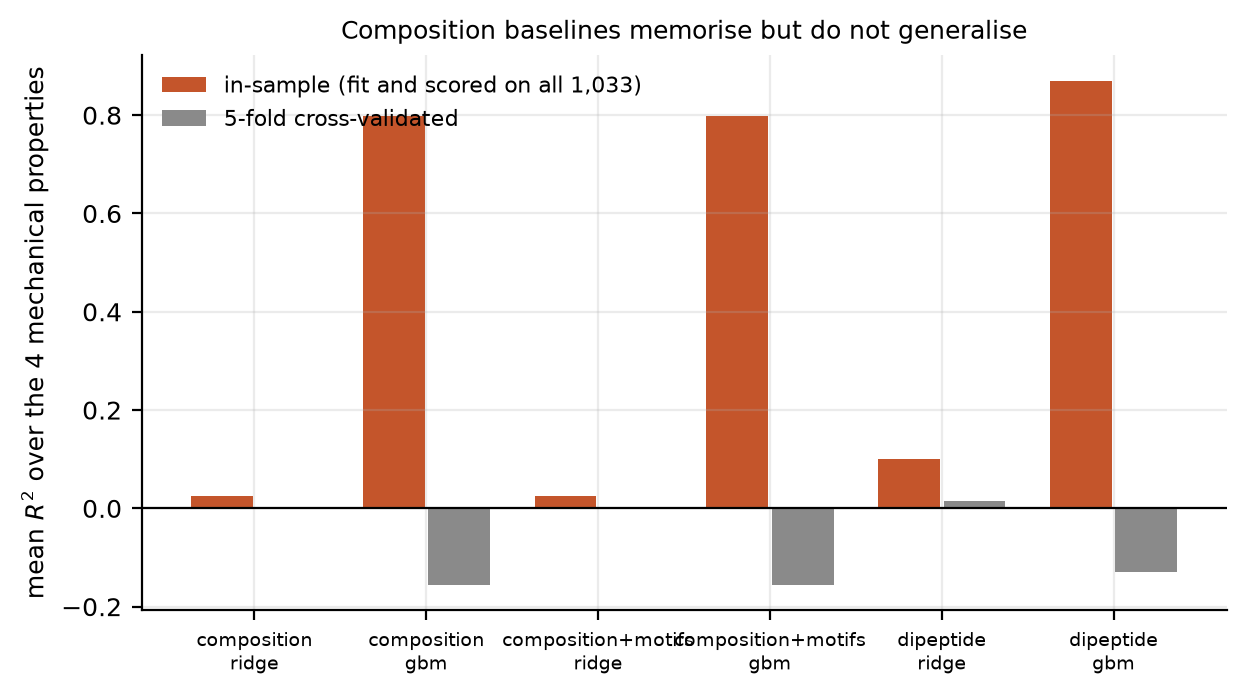
\includegraphics[width=0.88\linewidth]{figures/fig5_baseline.png}
\caption[Baseline]{\textbf{Composition baselines memorise but do not
generalise.} Each pair of bars is one feature set and model. Orange is
in-sample (fit and scored on all 1{,}033 rows); grey is 5-fold
cross-validated. Gradient boosting reaches $R^2 \approx 0.80$--$0.87$ in-sample
and \emph{negative} under cross-validation --- worse than predicting the dataset
mean. The gap between the two bars is the entire point of the figure.}
\label{fig:baseline}
\end{figure}

\begin{table}[htbp]
\centering\small
\caption[Baseline numbers]{Mean \Rsq{} over the four mechanical properties.}
\begin{tabular}{llcc}
\toprule
\textbf{features} & \textbf{model} & \textbf{in-sample} & \textbf{5-fold CV} \\
\midrule
composition & ridge & 0.026 & 0.001 \\
composition & GBM & \textbf{0.799} & \textbf{$-0.155$} \\
composition + motifs & ridge & 0.025 & 0.004 \\
composition + motifs & GBM & 0.798 & $-0.155$ \\
dipeptide & ridge & 0.100 & 0.014 \\
dipeptide & GBM & 0.870 & $-0.130$ \\
\bottomrule
\end{tabular}
\end{table}

Species-grouped cross-validation, where no species appears in both training and
test folds, gives $-0.049$.

\begin{goodbox}{Result}
On this dataset, in-sample fit and generalisation are close to \emph{unrelated}.
A model can reach 0.87 in-sample while being worse than useless out of sample.
Since the paper fine-tunes on all 1{,}033 pairs and holds nothing out, that
warning applies to any forward-task accuracy measured on them --- the paper's
and mine alike.
\end{goodbox}

\subsection{The baseline on Table 1's own axis}

Scoring the same baseline the paper's way --- within-vector \Rsq, one value per
sequence --- puts it on the only axis directly comparable to the headline
numbers:

\begin{center}
\small
\begin{tabular}{lc}
\toprule
composition ridge on real pairs & mean $-1.70$, median $-0.22$, \textbf{max 0.697} \\
paper, eight targets & 0.564 -- 0.890 \\
this project, eight targets & 0.223 -- 0.722 \\
\bottomrule
\end{tabular}
\end{center}

\begin{warnbox}{Not a like-for-like comparison}
The baseline figure is the maximum over 1{,}033 \emph{in-sample fits} to
sequences whose labels it trained on. The paper's is the maximum over $\sim$2{,}000
\emph{generated} sequences scored against a target never in any training set.
Different procedures, different denominators.

What the number does show is that a value in the 0.6--0.7 band \emph{on this
metric} is reachable without a transformer and without generation --- worth
knowing before reading any single such value as evidence of sequence
understanding.
\end{warnbox}

\section{Extension 4: what happens outside MaSp?}
\label{sec:nonmasp}

The model is fine-tuned on MaSp only. The database contains seven other
spidroin families from the same individuals. The forward task accepts them
without complaint.

\begin{figure}[htbp]
\centering
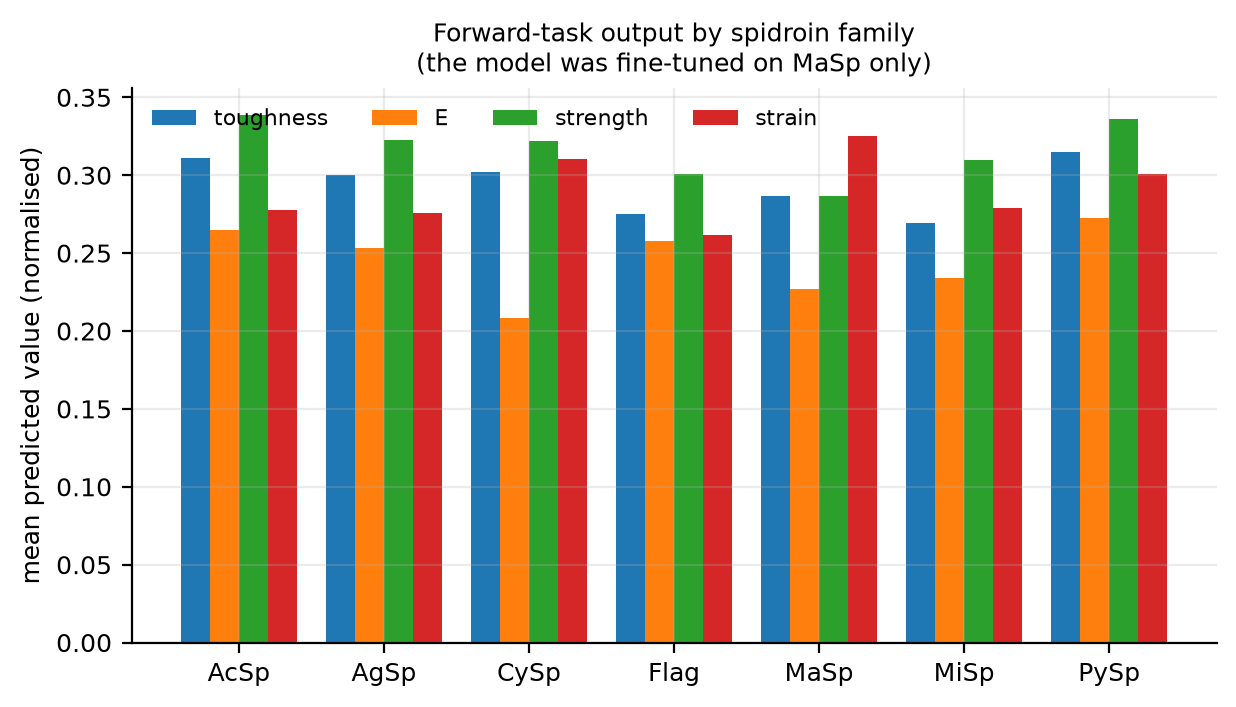
\includegraphics[width=0.88\linewidth]{figures/fig6_nonmasp.png}
\caption[Non-MaSp predictions]{\textbf{Mean prediction by spidroin family.}
Four bars per family, one per mechanical property. If the model were reading
the sequence deeply, families as different as Flag (the stretchy capture
spiral) and MaSp (the stiff dragline) should look different. They barely do ---
every family's bars sit at nearly the same heights.}
\label{fig:nonmasp}
\end{figure}

\begin{table}[htbp]
\centering\small
\caption[Accuracy by family]{Accuracy against measured dragline properties.}
\begin{tabular}{lccc}
\toprule
\textbf{family} & \textbf{in training?} & \textbf{mean \Rsq} & \textbf{mean abs.\ error} \\
\midrule
MaSp & \textbf{yes} & \textbf{$+0.826$} & 0.024 \\
MiSp & no & $-0.270$ & 0.141 \\
AcSp & no & $-0.317$ & 0.170 \\
AgSp & no & $-0.430$ & 0.158 \\
CySp & no & $-0.472$ & 0.151 \\
Flag & no & $-0.514$ & 0.161 \\
PySp & no & $-0.540$ & 0.152 \\
\bottomrule
\end{tabular}
\end{table}

Accuracy falls off a cliff outside MaSp, from $+0.83$ to between $-0.27$ and
$-0.54$, with error rising six-fold.

And the predictions barely depend on family at all. The between-family spread of
the mean prediction is \textbf{0.019} against a within-family spread of
\textbf{0.095} --- a ratio of \textbf{0.199}, both measured over the same four
mechanical properties.

\begin{goodbox}{Result}
Handed a spidroin it has not memorised, the model emits something close to its
training marginal regardless of which silk family the sequence came from.
\end{goodbox}

\begin{warnbox}{The caveat, stated before the numbers are used}
Silkome's mechanical properties are measured on \emph{dragline}, which is MaSp.
A Flag sequence here is paired with the same spider's dragline properties, not
with flagelliform properties. So this is \emph{not} a test of whether the model
can predict flagelliform silk --- no analysis of this dataset could be. It is
the narrower question of whether a non-MaSp sequence from an individual still
recovers that individual's dragline properties.

The between/within ratio needs no such caveat: it uses no ground truth at all.
\end{warnbox}

\section{The thing all four extensions point at}
\label{sec:memorisation}

Four independent measurements converge.

\subsection{The forward task returns training labels verbatim}

Over the 1{,}033 fine-tuning pairs, the forward task's in-sample \Rsq{} averages
0.696 across the four mechanical properties. Respectable. But:

\begin{goodbox}{732 of 1{,}026 scored rows --- 71.3\% --- come back with all eight
values \emph{identical} to the training label}
to within 0.0005, which is the resolution the model can express. Mean absolute
error on those rows is 0.00025. On the remaining 294 rows it is 0.109, and the
mean \Rsq{} is $\mathbf{-0.113}$: worse than predicting the dataset mean.
\end{goodbox}

\begin{figure}[htbp]
\centering
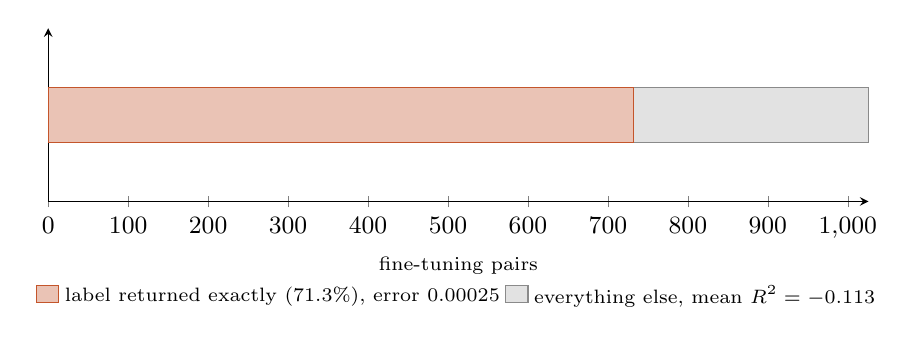
\begin{tikzpicture}[font=\small]
\begin{axis}[
  width=12cm,height=4.4cm,
  xbar stacked, xmin=0, xmax=1026,
  ytick=\empty, y=1.1cm,
  xlabel={fine-tuning pairs}, xlabel style={font=\scriptsize},
  bar width=0.7cm, axis lines=left,
  legend style={font=\scriptsize,draw=none,at={(0.5,-0.42)},anchor=north,legend columns=2},
  clip=false,
]
\addplot[fill=ourscol!35,draw=ourscol] coordinates {(732,0)};
\addlegendentry{label returned exactly (71.3\%), error 0.00025}
\addplot[fill=greyc!25,draw=greyc] coordinates {(294,0)};
\addlegendentry{everything else, mean $R^2 = -0.113$}
\end{axis}
\end{tikzpicture}
\caption[Memorisation]{The composition of the in-sample \Rsq{} of 0.696. Most
of it rests on rows where the model returned the training label verbatim rather
than predicting anything.}
\label{fig:memorisation}
\end{figure}

\subsection{The inverse task returns training sequences verbatim}
\label{sec:regurgitation}

\begin{center}
\small
\begin{tabular}{lccc}
\toprule
\textbf{set} & \textbf{parsed} & \textbf{verbatim copies} & \textbf{copy rate} \\
\midrule
F1 & 1946 & 1122 & 57.7\% \\
F2 & 1961 & 1219 & 62.2\% \\
F3 & 1949 & 1208 & 62.0\% \\
S1 & 1953 & 1237 & 63.3\% \\
S2 & 1948 & 1206 & 61.9\% \\
S3 & 1955 & 1194 & 61.1\% \\
S4 & 1958 & 1243 & 63.5\% \\
S5 & 1974 & 1324 & 67.1\% \\
\midrule
\textbf{overall} & & & \textbf{62.3\%} \\
\bottomrule
\end{tabular}
\end{center}

Nearly two thirds of generations are byte-identical to sequences in the
reference set. These are not a handful of repeats --- 200 to 290 \emph{distinct}
known sequences appear per set. A nominal budget of 2{,}048 therefore yields
about 771 scoreable candidates.

This contradicts nothing in the paper, which analyses only the novel outputs.
But the discard rate is not reported, and it means the model's default
behaviour in the inverse direction includes a great deal of retrieval.

\subsection{Putting it together}

\begin{keybox}{The picture}
\begin{itemize}[leftmargin=*,itemsep=2pt]
  \item Forward: returns the exact training label 71\% of the time; on the rest,
        worse than the mean.
  \item Inverse: returns a verbatim training sequence 62\% of the time.
  \item Outside its training family: accuracy collapses, $+0.83 \to -0.27\ldots-0.54$.
  \item Its output barely varies with family: ratio 0.199.
  \item A composition baseline shows the underlying task is genuinely hard ---
        cross-validated \Rsq{} near zero.
\end{itemize}
The pipeline behaves substantially like a \emph{retrieval system} over its
fine-tuning set, in both directions.
\end{keybox}

\begin{warnbox}{Three qualifications, because this invites overreading}
\textbf{It contradicts nothing the paper claims.} The paper fine-tunes on all
pairs, says so, reports self-consistency rather than held-out accuracy, and
makes no generalisation claim. Memorisation is the \emph{expected} consequence
of training on everything and evaluating on the same data.

\textbf{The $-0.113$ is not a generalisation estimate.} Those rows are selected
on the outcome, and they differ systematically from the rest --- median length
456 against 361. Selecting on the outcome biases the estimate downward by an
unknown amount. A real held-out number requires retraining with a fold held
out, which I did not do.

\textbf{The task is genuinely hard.} The composition baseline establishes that
nobody --- not the transformer, not ridge regression --- has demonstrated
generalisation on this dataset. That is a property of the problem, not of any
particular model.
\end{warnbox}

\section{The reproduction of Table 1, seen whole}

\begin{figure}[htbp]
\centering
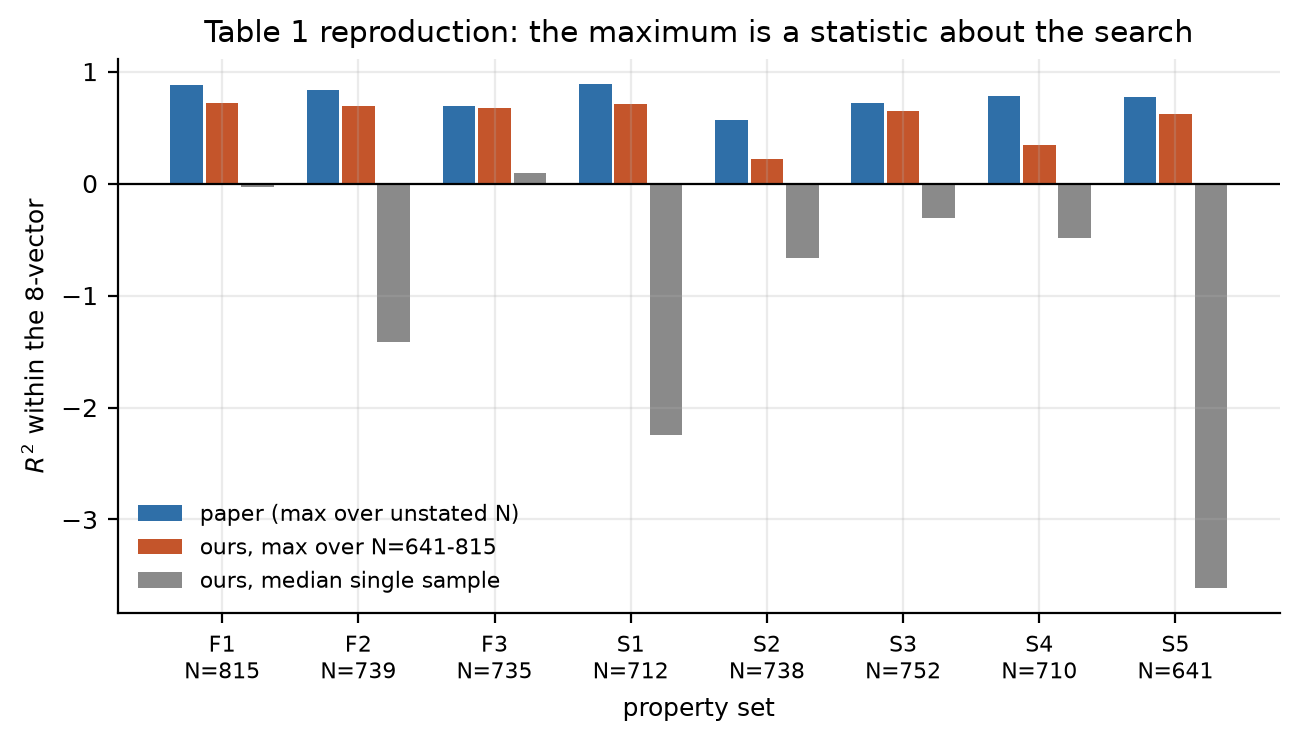
\includegraphics[width=\linewidth]{figures/fig1_table1_reproduction.png}
\caption[Table 1 reproduction]{\textbf{The headline comparison.} For each
target: blue is the paper's published \Rsq{} (a maximum over an unstated $N$),
orange is my pool maximum, grey is my \emph{median} single candidate. The tick
labels give each set's scoreable pool size. The orange bars fall short
everywhere --- that is the shortfall of Section~\ref{sec:table1}, now known to
live in the search rather than the model. The grey bars are the more
informative ones: they show what a single draw from this pipeline is typically
worth, and for six of eight targets that is below zero.}
\label{fig:table1}
\end{figure}

\chapter{Three things I got wrong}
\label{ch:mistakes}

Three times I stated a result and had to withdraw it. This chapter is not
penance --- the pattern across the three turned out to be the most transferable
thing in the project, and all three are instructive in different ways.

\section{Retraction 1: a sign discrepancy that was not there}
\label{sec:d13}

\paragraph{The claim.} The paper's motif table (Table~S4) defines fourteen
short sequence motifs, each tagged as increasing or decreasing a mechanical
property, and states they were ``selected and concluded from Table 1'' of the
Silkome paper. I compared the two and reported that \emph{three} motifs carried
the opposite sign to their cited source --- including \aaseq{GQ}, which the paper
uses to support a conclusion about high-modulus designs.

That is a serious thing to say about a published paper.

\paragraph{What actually happened.} I had read the Silkome Table 1 via automated
retrieval of a web page --- twice, by different routes, which agreed. Both were
wrong in the same way.

\begin{figure}[htbp]
\centering
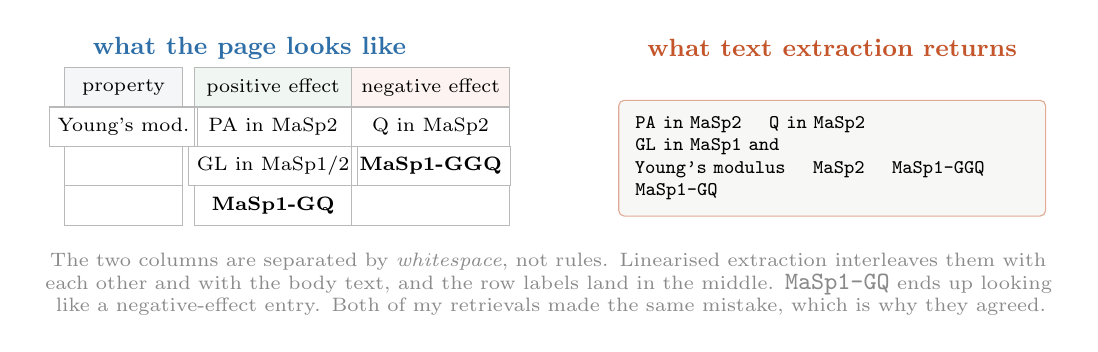
\begin{tikzpicture}[font=\scriptsize,
  cell/.style={draw=greyc!60,minimum height=0.5cm,inner sep=3pt},
]
% left: the real table
\node[font=\small\bfseries,text=papercol] at (2.6,2.5) {what the page looks like};
\node[cell,minimum width=1.5cm,fill=boxbg] at (1.0,2.0) {property};
\node[cell,minimum width=2.0cm,fill=goodbg] at (2.9,2.0) {positive effect};
\node[cell,minimum width=2.0cm,fill=warnbg] at (4.9,2.0) {negative effect};
\node[cell,minimum width=1.5cm] at (1.0,1.5) {Young's mod.};
\node[cell,minimum width=2.0cm] at (2.9,1.5) {PA in MaSp2};
\node[cell,minimum width=2.0cm] at (4.9,1.5) {Q in MaSp2};
\node[cell,minimum width=1.5cm] at (1.0,1.0) {};
\node[cell,minimum width=2.0cm] at (2.9,1.0) {GL in MaSp1/2};
\node[cell,minimum width=2.0cm] at (4.9,1.0) {\textbf{MaSp1-GGQ}};
\node[cell,minimum width=1.5cm] at (1.0,0.5) {};
\node[cell,minimum width=2.0cm] at (2.9,0.5) {\textbf{MaSp1-GQ}};
\node[cell,minimum width=2.0cm] at (4.9,0.5) {};

% right: linearised
\node[font=\small\bfseries,text=ourscol] at (10.0,2.5) {what text extraction returns};
\node[draw=ourscol!50,fill=codebg,rounded corners=2pt,inner sep=6pt,
      text width=5.0cm,font=\ttfamily\scriptsize,align=left] at (10.0,1.1)
  {PA in MaSp2 \quad Q in MaSp2\\
   GL in MaSp1 and\\
   Young's modulus \quad MaSp2 \quad MaSp1-GGQ\\
   MaSp1-GQ};

\node[text width=13cm,align=center,font=\scriptsize,text=greyc] at (6.4,-0.5)
  {The two columns are separated by \emph{whitespace}, not rules. Linearised
   extraction interleaves them with each other and with the body text, and the
   row labels land in the middle. \aaseq{MaSp1-GQ} ends up looking like a
   negative-effect entry. Both of my retrievals made the same mistake, which is
   why they agreed.};
\end{tikzpicture}
\caption[The column-interleaving failure]{How a two-column table becomes a
false finding.}
\label{fig:d13}
\end{figure}

\paragraph{The fix.} Rendering the page as an \emph{image} and reading it
visually resolves it in one look. Silkome Table 1 lists \aaseq{QGP} and
\aaseq{PGA} as \emph{positive} for strain at break and \aaseq{MaSp1-GQ} as
\emph{positive} for Young's modulus --- exactly what Table~S4 says. All fourteen
entries agree with their source. The paper's transcription is faithful.

\begin{warnbox}{What I should have done}
The original entry did flag that it rested on a web fetch and recommended
checking the source directly. That was right, and doing so is what overturned
it --- but I should not have published the claim in that state at all. A claim
that a published paper contradicts its own source has a higher evidence bar than
a claim about my own measurements, because the cost of being wrong falls on
someone else.
\end{warnbox}

\section{Retraction 2: corrupted sequences that passed every length check}
\label{sec:tables1}

\paragraph{The claim.} Having extracted the paper's own generated sequences
from Table~S1, I ran them through the forward task and got \Rsq{} values far
\emph{below} the published ones. That would have read as the paper failing on
its own specimens.

\paragraph{Why the extraction was wrong.} Table~S1 spans four PDF pages. My
first extractor used the table's ruling rectangles to find row boundaries. The
subtlety: the ID cell is vertically \emph{centred} in its row, so in linear text
the ID appears in the middle of the sequence it labels, and long sequences span
page breaks.

\begin{figure}[htbp]
\centering
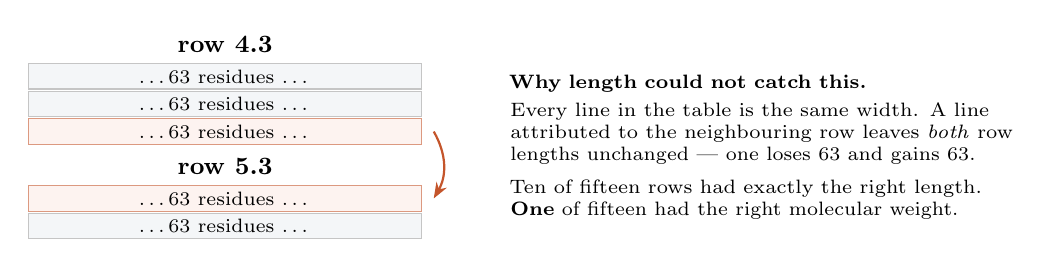
\begin{tikzpicture}[font=\scriptsize,
  ln/.style={draw=greyc!50,fill=boxbg,minimum width=5.0cm,minimum height=0.32cm,
             inner sep=1pt},
  bad/.style={ln,fill=warnbg,draw=ourscol!60},
]
\node[font=\small\bfseries] at (2.5,2.3) {row 4.3};
\node[ln] at (2.5,1.9) {\ldots 63 residues \ldots};
\node[ln] at (2.5,1.55) {\ldots 63 residues \ldots};
\node[bad] at (2.5,1.2) {\ldots 63 residues \ldots};
\draw[ourscol,-{Stealth[length=2mm]},thick] (5.15,1.2) to[bend left=30] (5.15,0.35);

\node[font=\small\bfseries] at (2.5,0.75) {row 5.3};
\node[bad] at (2.5,0.35) {\ldots 63 residues \ldots};
\node[ln] at (2.5,0.0) {\ldots 63 residues \ldots};

\node[text width=6.4cm,align=left,font=\scriptsize,anchor=west] at (6.0,1.0)
  {\textbf{Why length could not catch this.}\\[2pt]
   Every line in the table is the same width. A line attributed to the
   neighbouring row leaves \emph{both} row lengths unchanged --- one loses 63
   and gains 63.\\[4pt]
   Ten of fifteen rows had exactly the right length. \textbf{One} of fifteen had
   the right molecular weight.};
\end{tikzpicture}
\caption[The line-misattribution failure]{Uniform line width makes length a
useless check. Molecular weight, which depends on every residue identity rather
than the count, catches it immediately.}
\label{fig:s1bug}
\end{figure}

\paragraph{The diagnostic that caught it.} Table~S3 publishes both the
\emph{length} and the \emph{molecular weight} of all fifteen sequences.

\begin{center}
\small
\begin{tabular}{lc}
\toprule
length check & 10/15 passed \\
molecular weight check & \textbf{1/15} passed \\
\bottomrule
\end{tabular}
\end{center}

Had I only checked length --- the obvious check --- ten of fifteen rows would have
passed and I would have published a dramatic, wrong claim about the paper
failing on its own data.

\paragraph{The rewrite.} Three patches failed. What worked was abandoning the
approach: ignore the ruling rectangles entirely, read every glyph in the
sequence column, group into lines, filter to residue-only lines by content,
concatenate in document order, and cut at the \emph{published lengths} in the ID
order. Since published lengths are now an input, length can no longer verify
anything --- molecular weight does, and it is independent of the split criterion.

\begin{goodbox}{Result after the rewrite}
Total 18{,}844 residues, exactly the Table~S3 sum. \textbf{13 of 13 checkable
rows match their published molecular weight to the cent.} The other two contain
\aaseq{X} codes that Biopython cannot weigh; they are length-exact and bracketed
by verified rows.

And the corrected forward-task result is the \emph{opposite} of the retracted
one: exact agreement on four of five sets (Section~\ref{sec:exactmatch}).
\end{goodbox}

One further detail cost 74 residues before it was found: the last line of each
sequence is a partial one, sometimes only a few residues, and a 20-character
minimum line length silently discarded them. No length threshold is needed --- the
residue-only alphabet test alone separates sequence lines from captions,
headers and page numbers, all of which contain lowercase or digits.

\section{Retraction 3: an analysis that could not fail}
\label{sec:nullretraction}

\paragraph{The claim.} A composition analysis --- rank spiders by each mechanical
property, compare the top ten against the bottom ten, find which residues differ
most --- recovered 12 of the 14 residues a related paper reports, under
\emph{both} of two amino-acid grouping schemes. I presented that as convergent
evidence.

\paragraph{Why it was worthless.} The selection rule takes the top $k$ residues
from each of three groups. With $k = 5$ and groups of 4--6 members, every
charged residue is selected \emph{automatically}, whatever the data says. The
rule picks 17.8 of 20 residues on average.

\begin{figure}[htbp]
\centering
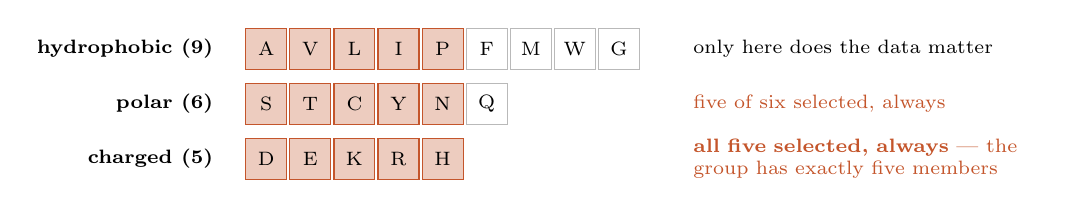
\begin{tikzpicture}[font=\small,
  aa/.style={draw=greyc!60,minimum width=0.52cm,minimum height=0.52cm,
             font=\scriptsize,inner sep=1pt},
  sel/.style={aa,fill=ourscol!30,draw=ourscol},
]
\node[font=\scriptsize\bfseries,anchor=east] at (-0.25,0) {hydrophobic (9)};
\foreach \i/\l in {0/A,1/V,2/L,3/I,4/P} { \node[sel] at (0.3+0.56*\i,0) {\l}; }
\foreach \i/\l in {5/F,6/M,7/W,8/G}     { \node[aa]  at (0.3+0.56*\i,0) {\l}; }

\node[font=\scriptsize\bfseries,anchor=east] at (-0.25,-0.7) {polar (6)};
\foreach \i/\l in {0/S,1/T,2/C,3/Y,4/N} { \node[sel] at (0.3+0.56*\i,-0.7) {\l}; }
\foreach \i/\l in {5/Q}                 { \node[aa]  at (0.3+0.56*\i,-0.7) {\l}; }

\node[font=\scriptsize\bfseries,anchor=east] at (-0.25,-1.4) {charged (5)};
\foreach \i/\l in {0/D,1/E,2/K,3/R,4/H} { \node[sel] at (0.3+0.56*\i,-1.4) {\l}; }

\node[anchor=west,font=\scriptsize,text=ourscol,text width=4.4cm] at (5.6,-1.4)
  {\textbf{all five selected, always} --- the group has exactly five members};
\node[anchor=west,font=\scriptsize,text=ourscol,text width=4.4cm] at (5.6,-0.7)
  {five of six selected, always};
\node[anchor=west,font=\scriptsize,text width=4.4cm] at (5.6,0)
  {only here does the data matter};
\end{tikzpicture}
\caption[The selection artifact]{Top-5-per-group selection when the groups have
9, 6 and 5 members. Orange is selected. Ten of the twenty residues are chosen
before the data is consulted.}
\label{fig:selectionbug}
\end{figure}

\paragraph{The null that killed it.} Apply the identical selection rule to
\emph{uniform random} values, 2{,}000 times:

\begin{center}
\small
\begin{tabular}{lcc}
\toprule
& \textbf{recovers of 14} & \textbf{selects of 20} \\
\midrule
random noise, scheme A & \textbf{12.7} & 17.8 \\
random noise, scheme B & 12.1 & 16.8 \\
\emph{my real data} & \emph{12} & --- \\
\bottomrule
\end{tabular}
\end{center}

Random data scores \emph{better} than the real data. The statistic carried no
information whatsoever.

\paragraph{The corrected analysis.} With the rule tightened to two per group and
a permutation null reported alongside every observed value:

\begin{center}
\small
\begin{tabular}{lccc}
\toprule
\textbf{scheme} & \textbf{observed} & \textbf{null} & \textbf{$p$} \\
\midrule
A & 5/14 & 5.3/14 & \textbf{0.75} \\
B & 5/14 & 5.5/14 & \textbf{0.79} \\
\bottomrule
\end{tabular}
\end{center}

\begin{goodbox}{The honest result is negative}
At this dataset size and with this method, the composition signal is not
distinguishable from chance.
\end{goodbox}

\begin{warnbox}{The part that stings}
I had built a careful two-scheme sensitivity analysis around a \emph{secondary}
ambiguity --- the amino-acid grouping, which genuinely is unspecified in the
source --- while the \emph{primary} statistic was vacuous. Check that an analysis
can fail before checking how sensitive it is to its assumptions.
\end{warnbox}

\section{Retraction 4, of a sort: being unfair to myself}
\label{sec:d8}

Not a retraction of a result, but of an attribution, and it went the other way.

The paper's Experimental Section prints a worked example sequence. My
transcription came to 635 residues and was not a byte-identical match to
anything in the database. I wrote that off as \emph{my} PDF extraction losing
characters across line wraps.

Checking it properly:

\begin{center}
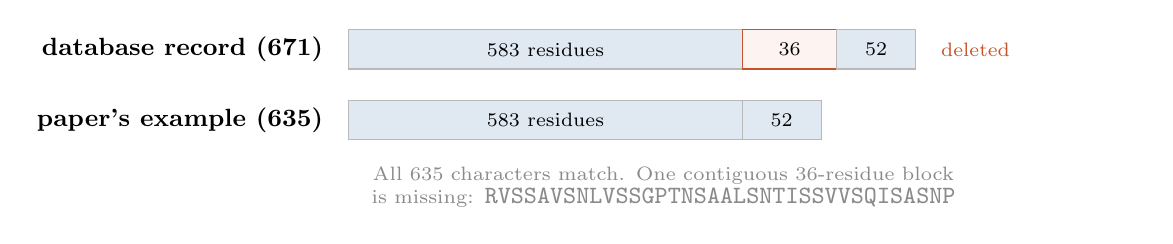
\begin{tikzpicture}[font=\scriptsize,
  seg/.style={draw=greyc!60,minimum height=0.5cm,inner sep=2pt},
]
\node[font=\small\bfseries,anchor=east] at (-0.2,0.55) {database record (671)};
\node[seg,minimum width=5.0cm,fill=papercol!15] at (2.5,0.55) {583 residues};
\node[seg,minimum width=1.2cm,fill=warnbg,draw=ourscol] at (5.6,0.55) {36};
\node[seg,minimum width=1.0cm,fill=papercol!15] at (6.7,0.55) {52};

\node[font=\small\bfseries,anchor=east] at (-0.2,-0.35) {paper's example (635)};
\node[seg,minimum width=5.0cm,fill=papercol!15] at (2.5,-0.35) {583 residues};
\node[seg,minimum width=1.0cm,fill=papercol!15] at (5.5,-0.35) {52};

\node[anchor=west,font=\scriptsize,text=ourscol] at (7.4,0.55) {deleted};
\node[text width=12cm,align=center,font=\scriptsize,text=greyc] at (4.0,-1.2)
  {All 635 characters match. One contiguous 36-residue block is missing:
   \aaseq{RVSSAVSNLVSSGPTNSAALSNTISSVVSQISASNP}};
\end{tikzpicture}
\end{center}

My transcription is \textbf{byte-exact}. The paper prints two variants of one
record --- the inverse-task example matches the database, the forward-task
example is that record minus a 36-residue block. Most likely a slip while
preparing the example; I state it neutrally and make no claim about which was
intended.

\begin{goodbox}{And it makes the check stronger}
Both variants return the published property vector from the forward task ---
the 635-residue printed example \emph{and} the full 671-residue database record.
So the model returns the published answer for a sequence that is \emph{not} the
database record and is missing 36 residues from it. Two known-answer tests
where I thought I had one, and a sharper statement than the hedge it replaced.
\end{goodbox}

\begin{keybox}{Standards cut both ways}
This project's discipline is about not being unfair to the paper. It should
equally be about not being unfair to my own tooling. Blaming my extraction for a
discrepancy \emph{without checking} is the same failure of accuracy as blaming
the paper would have been --- I simply chose the self-deprecating error instead
of the accusatory one, and felt virtuous doing it.
\end{keybox}

\section{The pattern}

\begin{keybox}{What the four have in common}
Every one of them:
\begin{enumerate}[leftmargin=*,itemsep=2pt]
  \item looked right,
  \item survived internal consistency checks,
  \item and was caught only by comparison against an \textbf{external published
        quantity that played no part in generating the claim}.
\end{enumerate}

The external quantities were: Silkome's own Table 1 read as an image; published
molecular weights; a permutation null; a sequence alignment.

The generalisable rule I take from this: \emph{for any claim that matters,
identify a quantity you did not use in producing it, and check against that.}
Internal consistency is necessary and nowhere near sufficient. My length check
passed 10/15 while the extraction was badly broken; my two web retrievals agreed
with each other while both were wrong.
\end{keybox}

This is also why the project has a test file whose entire job is checking that
the prose matches the code --- figure colour rules against the ablation names
actually emitted, README counts against the real counts, cross-references
against files that exist. Two of the bugs found in a later review would have
been caught by those tests, and now are.

\chapter{Reference}
\label{ch:reference}

\section{Conclusions, stated compactly}

\begin{description}[leftmargin=0cm,style=nextline,itemsep=6pt]

\item[What reproduces exactly.] The checkpoint is the model described
  (253{,}556{,}736 parameters). It returns the published property vector for the
  published worked example --- for both printed variants of it. The 1{,}033-pair
  dataset reconstructs to the exact published count. The normalisation constants
  were recovered independently and later confirmed against the real Table~S5,
  all eight. Given the paper's own designed sequences, the forward task returns
  the published \Rsq{} to four decimals on four of five sets, matching the whole
  predicted vector slot for slot. Descriptors match on 15/15 molecular weights
  and isoelectric points.

\item[What reproduces partially.] Running the design procedure end to end, my
  maximum falls below the published value on all eight targets, mean gap 0.27.
  Because the scorer reproduces exactly, this is located in the inverse task's
  \emph{search}, not in the model. Why the authors' search found longer and
  better candidates, I cannot say.

\item[What the numbers measure.] The headline \Rsq{} is a maximum over a
  sampling budget that is not stated, of a within-vector self-consistency
  measure, from a model that returns the exact training label for 71\% of its
  fine-tuning pairs and emits verbatim training sequences 62\% of the time.
  Each qualifier is individually reasonable; together they mean the number
  measures something narrower than it appears to.

\item[What would remove the ambiguity.] Two changes, neither requiring new
  experiments: state $N$ alongside any best-of-$N$ result, and hold out a fold.
  On 1{,}033 pairs a held-out fold is cheap, and the baselines suggest it would
  be informative --- the gap between in-sample and cross-validated performance on
  this data is the difference between 0.80 and $-0.16$.

\item[The wider point.] Generative design pipelines that chain an inverse task
  into a forward task and report the agreement are measuring something real.
  But what they measure depends on the search budget and on how much of the
  training set the model has retained. Both are cheap to report and usually are
  not.

\end{description}

\section{The fifteen assumptions}

Every choice the paper does not specify. Full reasoning in
\code{ASSUMPTIONS.md}.

\begin{longtable}{@{}p{0.7cm}p{6.0cm}p{7.4cm}@{}}
\toprule
\textbf{ID} & \textbf{the choice} & \textbf{basis} \\
\midrule
\endhead
A1 & Dataset reconstruction rule & Join on \code{idv\_id}; lands on 1{,}033 exactly \\
A2 & Normalisation constants & Recovered; verified 0.00047, later confirmed vs Table~S5 \\
A3 & Validity filter on generations & Twenty standard residues only; rejection rate reported \\
A4 & Definition of novelty & Paper's exact-match test, plus $k$-mer measures; calibrated in §\ref{sec:exactmatch} \\
A5 & Greedy forward decoding & 58/60 identical to sampled; batch-invariant \\
A6 & Inference precision & float16 on GPU; determinism verified at that precision \\
A7 & Terminal-domain boundaries & 130 / 100 residues, nominal literature values \\
A8 & Motif set & Superseded: Table~S4 obtained, all 14 entries verified \\
A9 & Sampling budget $N$ & Treated as a variable; the whole curve reported \\
A10 & Batched inference & Equivalence to unbatched tested \\
A11 & Checkpoint revision & Resolved commit recorded and pinnable \\
A12 & Duplicate sequence labels & Kept; the published count requires it \\
A13 & Composition accessor & Counted directly; avoids a Biopython API change \\
A14 & Secondary-structure convention & Both legacy and corrected reported (see D1) \\
A15 & Amino-acid grouping & Two schemes reported; neither chosen to fit \\
\bottomrule
\end{longtable}

\section{The fifteen discrepancies and open points}

\begin{longtable}{@{}p{0.7cm}p{6.0cm}p{7.4cm}@{}}
\toprule
\textbf{ID} & \textbf{point} & \textbf{status} \\
\midrule
\endhead
D1 & Figure 5c helix/sheet labels exchanged vs current Biopython & confirmed; upstream correction postdates publication \\
D2 & Set S3 strength 0.200 where the stated median is 0.310 & confirmed, internal to the paper \\
D3 & Sampling budget $N$ never stated & clarification; quantified in §\ref{sec:bestofn} \\
D4 & \Rsq{} is within-vector, not across a test set & clarification \\
D5 & No held-out set & clarification; stated by the paper itself \\
D6 & 62.3\% of generations are verbatim training sequences & confirmed \\
D7 & Supporting Information initially unobtainable & resolved via arXiv preprint \\
D8 & Paper prints two variants of one worked example & confirmed; my earlier self-blame retracted \\
D9 & \code{r2\_score} argument order differs between two helpers & clarification; no published number affected \\
D10 & Shortfall on all eight targets & confirmed; located in the search (§\ref{sec:exactmatch}) \\
D11 & Forward task returns 71\% of training labels verbatim & confirmed \\
D12 & A reviewer comment described a different paper's figure & clarification \\
D13 & \textbf{Withdrawn.} Alleged motif sign discrepancy & \textbf{retracted}; all 14 entries agree \\
D14 & Recovered constants match published Table~S5 exactly & confirmed \\
D15 & Table~S1 extraction & failed, then rewritten and verified \\
\bottomrule
\end{longtable}

\section{Where every number comes from}

\begin{longtable}{@{}p{6.6cm}p{7.5cm}@{}}
\toprule
\textbf{script} & \textbf{produces} \\
\midrule
\endhead
\code{00\_check\_env.py} & architecture check, pinned revision \\
\code{01\_smoke\_test.py} & both tasks end to end, cost projection \\
\code{01b\_forward\_decoding\_diagnostics.py} & the evidence for assumption A5 \\
\code{02\_reproduce\_table1.py} & the eight candidate pools (the long run) \\
\code{03\_build\_dataset.py} & the 1{,}033 pairs; normalisation check \\
\code{04\_forward\_eval\_dataset.py} & in-sample forward accuracy \\
\code{04b\_memorisation\_audit.py} & the 71.3\% figure \\
\code{05\_protein\_properties.py} & Figure 5 descriptors \\
\code{06\_motif\_analysis.py} & Figure 7 motifs \\
\code{07\_novelty\_audit.py} & the 62.3\% verbatim-copy rate \\
\code{08\_extract\_table\_s1.py} & the paper's own sequences, MW-verified \\
\code{09\_verify\_published\_sequences.py} & the exact-match result \\
\code{09b\_verify\_against\_tables\_s2\_s3.py} & descriptor and novelty cross-checks \\
\code{10\_ablation\_bestofn.py} & best-of-$N$ curves \\
\code{10b\_scoring\_stochasticity.py} & the rejected explanation for the gap \\
\code{11\_ablation\_sequence\_content.py} & the sequence ablations \\
\code{12\_baseline\_composition.py} & the composition baselines \\
\code{13\_extension\_nonmasp.py} & out-of-distribution families \\
\code{14\_composition\_association.py} & composition association + null \\
\code{99\_make\_figures.py} & all six figures, from saved results \\
\bottomrule
\end{longtable}

Every script writes a JSON manifest under \code{results/} recording the git
commit, working-tree cleanliness, model revision, seed, platform, GPU and the
version of every library used.

\section{Glossary}

\begin{description}[leftmargin=0cm,style=nextline,itemsep=3pt]
\item[Amino acid] One link in a protein chain; twenty kinds, written as letters.
\item[Attention] The mechanism by which each position in a transformer draws on
  every other, with learned, content-dependent weights.
\item[Autoregressive] Generating one token at a time, each conditioned on all
  previous ones.
\item[Best-of-$N$] Generating $N$ candidates and keeping the highest-scoring.
  The expected result rises with $N$ regardless of model quality.
\item[BPE] Byte-pair encoding; builds a vocabulary by repeatedly merging the
  most frequent adjacent pair.
\item[Decoding] Turning next-token probabilities into an actual choice: greedy,
  or sampling with temperature / top-$k$ / top-$p$.
\item[Dragline] The silk a spider hangs from; made of MaSp; the silk that gets
  mechanically tested.
\item[Fine-tuning] Further training of a pretrained model on a specific task.
\item[Held-out] Data withheld from training, used to measure generalisation.
  There is none here.
\item[In-sample] Measured on training data. An upper bound, not an estimate.
\item[Instability index] A ProtParam statistic computed from dipeptide
  frequencies; estimates whether a protein is stable.
\item[Isoelectric point] The pH at which a protein carries no net charge.
\item[MaSp] Major ampullate spidroin; the dragline protein; the paper's subject.
\item[Motif] A short recurring sequence pattern, e.g.\ poly-A, GGX, GPGXX.
\item[Normalisation] Mapping raw measurements to $[0,1]$ by min--max scaling.
\item[Parameter] One learned number in a model. 253.6 million here.
\item[pLDDT] AlphaFold2's per-residue confidence score. 40--60 is low.
\item[Poly-A] A run of alanines; forms $\beta$-sheet nanocrystals; supplies
  strength and stiffness.
\item[ProtParam] A standard tool computing descriptors from a sequence.
\item[\Rsq] $1 - \mathrm{SS}_{\text{res}}/\mathrm{SS}_{\text{tot}}$. Negative
  values mean worse than guessing the mean.
\item[RoPE] Rotary positional embedding; encodes position by rotation, so
  relative offsets are what the attention sees.
\item[Spidroin] A spider silk protein.
\item[Temperature] A decoding parameter rescaling the distribution; lower is
  more deterministic.
\item[Token] The unit a model consumes; here, a chunk of amino acids.
\item[Toughness] Energy absorbed per unit volume before breaking; the area
  under the stress--strain curve.
\item[Within-vector \Rsq] The paper's definition: \Rsq{} across the eight
  property entries of one sequence.
\end{description}

\section{Reproducing the reproduction}

\begin{lstlisting}[style=plain]
python -m venv .venv && .venv/Scripts/activate
pip install torch --index-url https://download.pytorch.org/whl/cu126
pip install -e ".[dev]"

git clone https://github.com/lamm-mit/SilkomeGPT _ref/SilkomeGPT-main
# plus the two Silkome files; see data/raw/README.md

python scripts/00_check_env.py
python scripts/03_build_dataset.py --fasta <fasta> --mech <csv>
python scripts/02_reproduce_table1.py --n 2048     # ~4.5 h on a 6 GB GPU
python scripts/99_make_figures.py
\end{lstlisting}

Two things deliberately do not ship: the Silkome primary data and the authors'
checkpoint, neither of which is mine to redistribute. Both are freely
available, and \code{data/raw/README.md} says exactly what to fetch.

\section*{Sources}
\addcontentsline{toc}{section}{Sources}

\begin{enumerate}[leftmargin=*,itemsep=2pt]
\item W.~Lu, D.~L.~Kaplan, M.~J.~Buehler. Generative Modeling, Design, and
  Analysis of Spider Silk Protein Sequences for Enhanced Mechanical Properties.
  \emph{Adv.\ Funct.\ Mater.} \textbf{34}, 2311324 (2024).
  \href{https://doi.org/10.1002/adfm.202311324}{doi:10.1002/adfm.202311324}.
  Preprint with the supplementary tables:
  \href{https://arxiv.org/abs/2309.10170}{arXiv:2309.10170}.
\item K.~Arakawa \emph{et al.} 1000 spider silkomes: linking sequences to silk
  physical properties. \emph{Sci.\ Adv.} \textbf{8}, eabo6043 (2022).
\item A.~Pandey, W.~Chen, S.~Keten. Primary sequence-based data-constrained
  machine learning framework to predict mechanical properties of the spider
  silk. \emph{Commun.\ Mater.} (2024). \emph{(Source of the composition
  analysis in §\ref{sec:nullretraction}, not of anything in Lu et al.)}
\item Released model and notebook:
  \href{https://github.com/lamm-mit/SilkomeGPT}{github.com/lamm-mit/SilkomeGPT},
  \href{https://huggingface.co/lamm-mit/SilkomeGPT}{huggingface.co/lamm-mit/SilkomeGPT}.
\end{enumerate}


\end{document}
